\documentclass{bookest}

\usepackage{hyperref}
\usepackage{amsmath}
\usepackage{amssymb}
\usepackage{amsthm}
\usepackage{graphics}
\usepackage{graphicx}
\usepackage{floatrow}
\usepackage{tikz}
\usepackage{color}
\usepackage{algorithm}
\usepackage{algorithmicx}
\usepackage{algpseudocode}
\usepackage{caption}
\usepackage{subcaption}
\usepackage{exercise}
\usepackage{chngcntr}
\usepackage{array, booktabs, blkarray}
\usepackage{varwidth}
\usepackage{multicol}
\usepackage{float}
\usepackage{eurosym}



\newcommand{\reals}{\mathbb{R}}
\newcommand{\integers}{\mathbb{Z}}
\newcommand{\symm}{\mathbb{S}}  % symmetric matrices

\newcommand{\ev}{\mathbb{E}} %expected value
\newcommand{\var}{\text{Var}} %variance
\newcommand{\prob}{\mathbb{P}} %probability

\newcommand{\uncset}{\mathcal{U}} % uncertainty set
\newcommand{\uncsetbox}{\overline{\uncset}}
\newcommand{\dist}{\mathbb{P}} % probability distribution
\newcommand{\ambset}{\mathcal{P}} %ambiguity set (distributionally robust optimization)
\newcommand{\keyunc}{\mathcal{Z}} %key uncertainty
\newcommand{\expected}{\mathbb{E}} % expected value

\newcommand{\rank}{\mathop{\bf rank}}
\newcommand{\tr}{\mathop{\bf tr}}
\newcommand{\diag}{\mathop{\bf diag}}
\renewcommand{\rank}{\mathop{\bf rank}}
\newcommand{\conv}{\mathop{\bf conv}}
\newcommand{\spans}{\mathop{\bf span}}
\newcommand{\nulls}{\mathop{\bf null}}
\newcommand{\clo}{\mathop{\bf clo}}
\newcommand{\ifff}{\Leftrightarrow}

\renewcommand{\det}{\mathop{\bf det}}
\newcommand{\proj}{\mathop{\bf proj}}
\newcommand{\argmin}{\mathop{\rm argmin}}
\newcommand{\argmax}{\mathop{\rm argmax}}
\newcommand{\epi}{\mathop{\bf epi}} % epigraph
\newcommand{\dom}{\mathop{\bf dom}} % domain
\newcommand{\intr}{\mathop{\bf int}}
\newcommand{\bou}{\mathop{\bf bou}}

\newcommand{\mini}{\mathop{\text{min.~}}}
\newcommand{\maxi}{\mathop{\text{max.~}}}
\newcommand{\minf}{\mathop{\text{minimize~}}}
\newcommand{\maxf}{\mathop{\text{maximize~}}}
\newcommand{\stnew}{\mathop{\text{s.t.:~}}}
\newcommand{\stf}{\mathop{\text{subject to:~}}}

\newcommand{\braces}[1]{\left\{ #1 \right \}}
\newcommand{\brackets}[1]{\left[ #1 \right]}
\newcommand{\floor}[1]{\lfloor #1 \rfloor}
\newcommand{\ceil}[1]{\lceil #1 \rceil}
\newcommand{\ol}[1]{\overline{ #1 }}
\newcommand{\norm}[1]{\vert\vert #1 \vert\vert}

\newcommand{\lb}{\linebreak}

\newtheorem{theorem}{Theorem}[chapter]
\newtheorem*{theorem*}{Theorem}
\newtheorem{proposition}[theorem]{Proposition}
\newtheorem*{remark}{Remark}
\newtheorem{assumption}[theorem]{Assumption}
\newtheorem{definition}[theorem]{Definition}
\newtheorem{lemma}[theorem]{Lemma}
\newtheorem{corollary}[theorem]{Corollary}


\definecolor{spring}{RGB}{170, 227, 145}
\definecolor{MidnightBlue}{RGB}{20, 0, 200}
\newcommand{\sidenote}[1]{\pdfmargincomment{#1}}
\newcommand{\highlight}[2]{\pdfmarkupcomment[markup=Highlight, color=spring]{#1}{#2}}

\parindent 0cm
\parskip 0.15cm
\topmargin 0.2cm
\oddsidemargin 1cm
\evensidemargin 0.5cm
\textwidth 15cm
\textheight 21cm
\definecolor{blue}{rgb}{0.23,0.58,0.89}


\begin{document}

	\input{cover}

	\tableofcontents
	
	\part{Robust Linear Optimization}
	
	\chapter{Uncertainty and Robustness} \label{chapter_1}
	\section{Sources of Uncertainty}

For many optimization problems, it is very likely that the model parameters like coefficients or right-hand sides are not highly accurate. We distinguish four different sources for this:
\begin{enumerate}
	\item Measurement error (Temperature, Pressure)
	\item Estimation error (future demands, uncertain costs)
	\item Implementation error (engineering, length)
	\item Inexact Data error (population, road networks in developing countries)
\end{enumerate}
Even small deviations (0.01\%) can lead to extreme violations of the constraints and thus infeasibility of the original optimal solution.

\section{Probability Theory and its Limitations}

Probability theory is the predominant theory of our time to model uncertainty. But in order to estimate a probability of a relatively simple event, we need to invoke a rather heavy machinery from complex analysis and inverse of transforms. Calculating expected values from arbitrary distributions is difficult, simulating them is complicated, and approximating them not accurate. Thus, we are unable to solve probability problems when dimensions increase. This is rooted in the fact that probability theory was developed starting in the 17th century up until the beginning of the 20th century, before computational tractability became an issue. Modern linear optimization had from the beginning of the field as an objective to solve multi-dimensional problems computationally. Given the success of this, it is natural to model uncertain phenomena using RO.

\section{The Building Blocks of Robust Optimization}

Kolmogorov, who introduced the basic axioms of modern probability theory, states about the limit laws: "All epistemological value of the theory of probability is based on this: that large-scale random phenomena in their collective action create strict, non-random regularity." The key building block for RO is that rather than assuming as primitives the axioms of probability theory, we assume as primitives the conclutions of probability theory, namely its limit laws. Thus, we do not describe uncertain quantities as random variables, but as variables who take values from an uncertainty set $\uncset$, constructed with the underlying probability information.

\section{Classes of RO Problems}

There are three core problems we address: RO, ARO and DRO. The starting point is an optimization problem with uncertain parameters

\begin{align*}
	\min \{f(x) \mid f_i(z,x)\leq0,\;\forall i\in[m]\},
\end{align*}
where $x\in\reals^{n_x}$ is the decision vector, $z\in\reals^{n_z}$ is an uncertain parameter vector, and $f_i(\cdot,x)$ is assumed to be convex for all $x$.

\subsection{Robust optimization}
In Robust optimization, $\uncset$ is a convex compact uncertainty set and the constraints are to hold for all $z\in\uncset$, i.e., $x$ has to be robust feasible:
\begin{align}\label{p1c1:ROproblem}
	\min \{f(x) \mid f_i(z,x)\leq0,\;\forall z\in\uncset,\;\forall i\in[m]\}.
\end{align}
Because of the $\forall$-quantifier, for a contionuous uncertainty set, this problem has finitely many variables  and infinitely many constraints. The key computational issue is to reformulate problem \eqref{p1c1:ROproblem} to an equivalent, computationally tractable form.

\subsection{Adaptive robust optimization}

ARO differs from RO in that not all decisions are to be made \textit{here-and-now}, i.e., before any uncertain parameters become known. The \textit{wait-and-see} or adaptive decisions may be determined once some of the parameters are no longer uncertain. Since these decisions are functions of $z$, we denote them with $y(z)$. The adaptive problem can then be written as: 
\begin{align}\label{p1c1:ROproblem}
	\min \{f(x) \mid f_i(z,x,y(z))\leq0,\;\forall z\in\uncset,\;\forall i\in[m]\}.
\end{align}

\subsection{Distributionally robust optimization}

Instead of assuming uncertain values for $\tilde{z}$ like RO and ARO, DRO assumes an uncertan distribution $\dist_z$ for it. This distribution belongs to the ambiguity set $\ambset$. In this setting, there are two principal constraint types.

\textit{Worst-case expected feasibility} constraints ensure that the constraint is satisfied for the expected value of all possible distributions $\dist\in\ambset$:
\begin{align*}
	\min \{f(x) \mid \expected_{\dist_z} [f_i(\tilde{z},x)]\leq0,\;\forall \dist_z\in\ambset,\;\forall i\in[m]\}.
\end{align*}
The challenge herein is to obtain a tractable exact form of the worst-case expectation, or a good upper bound.

\textit{Chance constraints} ensure that constraints are satisfied with a certain probability for all $\dist\in\ambset$:
\begin{align*}
	\min \{f(x) \mid \dist_z\{f_i(\tilde{z},x)\leq0\}\geq 1-\epsilon,\;\forall \dist_z\in\ambset,\;\forall i\in[m]\}.
\end{align*}
Here, the challenge is to obtain a safe approximation, i.e., a computationally tractable system of constraints $\mathcal{S}$ that ensures feasibility for the above condition.


	
	\chapter{RO under Linear Uncertainty} \label{chapter_2}
	\section{Basics of linear problems}

As we have seen in the previous chapter, the feasible region of a linear programming problem can be represented as
%
\begin{equation} \label{p1c2:eq:feasible_region_inequality}
	Ax \leq b,	
\end{equation}
%
where $A$ is a $m \times n$ matrix, $x$ is a $n$-dimensional column vector (or more compactly, $x \in \reals^n$), and $b$ is an $m$-dimensional column vector ($b \in \reals^m$). Notice that $\leq$ is considered component-wise.

Before introducing the simplex method, let us first revisit a few key elements and operations that we will use in the process. The first of them is presented in Definition \ref{p1c2:def:matrix_inversion}.
%
\begin{definition}[Matrix inversion] \label{p1c2:def:matrix_inversion}
	Let $A$ be a square $n \times n$ matrix. $A^{-1}$ is the \emph{inverse matrix} of $A$ if it exists and $AA^{-1} = I$, where $I$ is the identity matrix.
\end{definition}
%
Matrix inversion is the ``kingpin'' of linear (and nonlinear) optimisation. As we will see later on, being able to perform efficient matrix inversion operations (in reality, operations that are equivalent to matrix inversion but that can exploit the matrix structure to be made faster) is of utmost importance for developing a linear optimisation solver. 

Another important concept is the notion of \emph{linear independence}. We formally state when a collection of vectors is said to be linearly independent (or dependent) in Definition \ref{p1c2:def:linear_independence}. 

%
\begin{definition}[Linearly Independent vectors] \label{p1c2:def:linear_independence}
	The vectors $\braces{x_i}_{i=1}^k \in \reals^n$  are \emph{linearly dependent} if there exist real numbers $\braces{a_i}_{i=1}^k$ with $a_i \neq 0$ for at least one $i \in \braces{1,\dots, k}$ such that
	$$
		\sum_{i=1}^k a_i x_i= 0;
	$$
	otherwise, $\braces{x_i}_{i=1}^k$ are linearly independent.
\end{definition}

In essence, for a collection of vectors to be linearly independent it must be so that none of the vectors in the collection can be expressed as a combination (that is multiplying the vectors by nonzero scalars and adding them) of the others. This is simpler to see in $\reals^2$. Two vectors are linearly independent if one cannot obtain one by multiplying the other by a constant, which, effectively, means that they are not parallel. If the two vectors are not parallel, then one of them must have a component in a direction that the other cannot achieve. The same holds for any $n$-dimensional space. Also, that is why one can only have up to $n$ independent vectors in $\reals^n$. Figure \ref{p1c2:fig:linear_independence} illustrates this effect. 

\begin{figure}[h]
	\centering
    \begin{tikzpicture}
%	        		\draw[help lines] (-2,-2) grid (2,3);
		\node (pic) at (0,0) {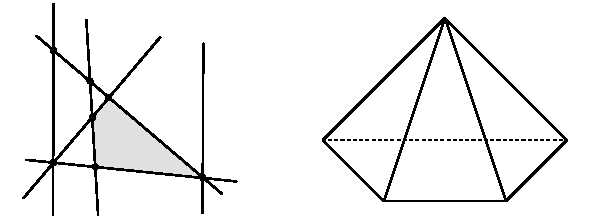
\includegraphics{part_1/chapter_2/figures/Figure1}};
		\node (x1) at (-1.7, 2.1) {$x_1$};
		\node (x2) at (1.2, 2.2) {$x_2$};
		\node (x11) at (-1.9, -0.2) {$x_1$};
		\node (x12) at (1, 0) {$x_2$};
		\node (x3) at (2.1, -0.8) {$x_3$};
    \end{tikzpicture}
	\caption{Linearly independent (top) and dependent (bottom) vectors in $\reals^2$}\label{p1c2:fig:linear_independence}
\end{figure}

Theorem \ref{p1c2:thm:fundamental_linear_algebra} summarises results that we will utilise in the upcoming developments. These are classical results from linear algebra and are thus provided without a proof.
%
\begin{theorem}[Inverses, linear independence, and solving $Ax = b$] \label{p1c2:thm:fundamental_linear_algebra}
	Let $A$ be a $m \times m$ matrix. Then, the following statements are equivalent:
	\begin{enumerate}
		\item $A$ is invertible
		\item $A^\top$ is invertible
		\item The determinant of $A$ is nonzero
		\item The rows of $A$ are linearly independent
		\item The columns of $A$ are linearly independent
		\item For every $b \in \reals^m$, the linear system $Ax = b$ has a unique solution
		\item There exists some $b \in \reals^m$ such that $Ax = b$ has a unique solution.	
	\end{enumerate}	
\end{theorem}
%
Notice that Theorem \ref{p1c2:thm:fundamental_linear_algebra} establishes important relationships between the geometry of the matrix $A$ (its rows and columns) and consequences it has to our ability to calculate its inverse $A^{-1}$ and, consequently, solve the system $Ax = b$, to which the solution is obtained as $x = A^{-1}b$. This will turn out to be most important operation in the simplex method.


\subsection{Subspaces and bases}

Let us define some objects that we will frequently refer to. The first of them is the notion of a \emph{subspace}. A subspace of $\reals^n$ is a set comprising all linear combinations of its own elements. Specifically, if $S$ is a subspace, then
%
\begin{equation*}
	S = \braces{ax + by : x,y \in S; a,b \in \reals}.
\end{equation*}
%
A related concept is the notion of a \emph{span}. A span of a collection of vectors $\braces{x_i}_{i=1}^k \in \reals^n$ is the subspace of $\reals^n$ formed by all linear combinations of such vectors, i.e., 
%
\begin{equation*}
	\spans(x_1,\dots, x_k) = \braces{y = \sum_{i=1}^k a_ix_i : a_i \in \reals, i \in \braces{1,\dots, k}}. 
\end{equation*}
%
Notice how the two concepts are related: subspaces can be characterised by a collection of vectors to which the span gives the said subspace. In other words, the span of a set of vectors is the subspace formed by all points we can represent by some linear combination of these vectors. 

The missing part in this is the notion of a \emph{basis}. A \emph{basis} of the subspace $S \subseteq \reals^n$ is a collection of vectors $\braces{x_i}_{i=1}^k \in \reals^n$ that are linearly independent such that $\spans(x_1,\dots, x_k) = S$. 

Notice that a basis is a ``minimal'' set of vectors that form a subspace. You can think of it in light of the definition of linearly independent vectors; if a vector is linearly dependent to the others, it is not needed for characterising the subspace the vectors span, since it can be represented by a linear combination of the other vectors (and thus is in the subspace formed by the span of the other vectors).

The above leads us to some important realisations:

\begin{enumerate}
	\item All bases of a given subspace $S$ have the same dimension. Any extra vector would be linearly dependent to those vectors that span $S$. In that case, we say that the subspace has size (or dimension) $k$, the number of linearly independent vectors forming the basis of the subspace.
	\item If the subspace $S \subset \reals^n$ is formed by a basis of size $m < n$, we say that $S$ is a proper subspace, because it is not the whole $\reals^n$ itself, but a space contained within $\reals^n$. For example, two linearly independent vectors form (i.e., span) a hyperplane in $\reals^3$; this hyperplane is a proper subspace since $m=2 <3=n$.
	\item If a proper subspace has dimension $m < n$, then it means that there are $n-m$ directions in $\reals^n$ that are perpendicular to the subspace and to each other. That is, there are nonzero vectors $a_i$ that are orthogonal to each other and to $S$. Or, equivalently, $a_i^\top x = 0$ for $i = n-m + 1, ..., n$. Referring to the $\reals^3$, if $m=2$, then there is a third direction that is perpendicular to (or not in) $S$. Figure \ref{p1c2:fig:proper_subpaces} illustrates this.
\end{enumerate}

\begin{figure}
	\centering
	\begin{tikzpicture}
%			\draw[help lines] (-4,-2) grid (4,2);
		\node (pic) at (0,0) {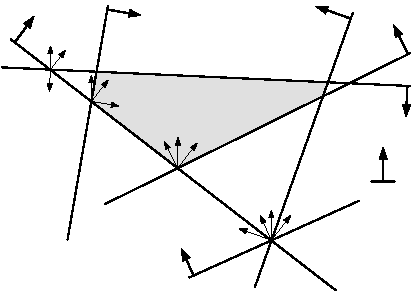
\includegraphics{part_1/chapter_2/figures/Figure2}};
		\node (x1l) at (-1.6, 0.6) {$x_1$};
		\node (Sl) at (-1.1, 0.9) {$S$};	
		\node (x1r) at (2.8, 0.8) {$x_1$};
		\node (x2r) at (2.6, -0.9) {$x_2$};
		\node (Sr) at (3.7, -0.3) {$S$};
	\end{tikzpicture}
	\vspace{-12pt}
	\caption{One- (left) and two-dimensional subspaces (right) in $\reals^3$} \label{p1c2:fig:proper_subpaces}
\end{figure}

Theorem \ref{p1c2:thm:LI_and_bases} builds upon the previous points to guarantee the existence of bases and propose a procedure to form them.

\begin{theorem}[Forming bases from linearly independent vectors]\label{p1c2:thm:LI_and_bases}
	Suppose that $S = \spans(x_1,\dots, x_k)$ has dimension $m \leq k$. Then
	\begin{enumerate}
		\item There exists a basis of $S$ consisting of $m$ of the vectors $x_1,\dots, x_k$.
		\item If $k' \leq m$ and $x_1,\dots, x_{k'} \in S$ are linearly independent, we can form a basis for $S$ by starting with $x_1,\dots, x_{k'}$ and choosing $m-{k'}$ additional vectors from $x_1,\dots, x_k$.
	\end{enumerate}	
\end{theorem}

%TODO: Include proof.

Our interest in subspaces and bases spans from (pun intended!) their usefulness in explaining how the simplex method works under a purely algebraic (as opposed to geometric) perspective. For now, we can use the opportunity to define some ``famous'' subspaces which will often appear in our derivations. 

Let $A$ be a $m \times n$ matrix as before. The \emph{column space} of $A$ consists of the subspace spanned by the $n$ columns of $A$ and has dimension $m$ (recall that each column has as many components as the number of rows and is thus a $m$-dimensional vector). Likewise, the \emph{row space} of $A$ is the subspace in $\reals^n$ spanned by the rows of $A$. Finally, the \emph{null space} of $A$, often denoted as $\nulls(A) = \braces{x \in \reals^n : Ax = 0}$, consist of the vectors that are perpendicular to the row space of $A$. 

One important notion related to those subspaces is that of their size. Both the row and the column space have the same size, and that size is the \emph{rank} of $A$. If $A$ is \emph{full rank}, than it means that 
%
\begin{equation*}
	\rank(A) = \min \braces{m,n}. 		
\end{equation*}
%
Finally, the size of the null space of $A$ is given $n - \rank(A)$, which is in line with Theorem \ref{p1c2:thm:LI_and_bases}.


\subsection{Affine subspaces}

A related concept is that of an \emph{affine subspace}. Differently from linear subspaces (to which we have been referring to simply as subspaces), affine subspaces encode some form of translation, such as  
%
\begin{equation*}
	S = S_0 + x_0 = \braces{x + x_0 : x \in S_0}.
\end{equation*}
%
Affine subspaces are not subspaces, because they do not contain the origin (recall that the definition of subspaces allows for $a$ and $b$ to be zero). Nevertheless, $S$ has the \emph{same dimension} as $S_0$.

Affine subspaces give a framework for representing linear programming problems algebraically. Specifically, let $A$ be a $m \times n$ matrix with $m < n$ (which will always be the case in linear programming models in this form as we will see) and $b$ a $m$-dimensional vector. Then, let 
%
\begin{equation} \label{p1c2:eq:equality_constraint_feasible_set}
	S = \braces{x \in \reals^n : Ax = b}.		
\end{equation}
%
As we will see, the feasible set of any linear programming problem can be represented as an equality-constrained equivalent of the form of \eqref{p1c2:eq:equality_constraint_feasible_set} by means of adding slack variables to the inequality constraints. Now, assume that $x_0 \in \reals^n$ is such that $Ax_0 = b$.  Then, we have that 
%
\begin{equation*}
	Ax = Ax_0 = b \Rightarrow A(x - x_0) = 0.	
\end{equation*}
%
Thus, $x \in S$ if and only if the vector $(x - x_0)$ belongs to $\nulls(A)$, the nullspace of $A$. Notice that the feasible region $S$ can be also defined as 
%
\begin{equation*}
	S = \braces{x + x_0 : x \in \nulls(A)},	
\end{equation*}
%
being thus an affine subspace with dimension $n-m$, if $A$ has $m$ linearly independent rows (i.e., $\rank(A)=m$). This will have important implications in the way we can define multiple basis from the $n$ vectors in the column space by choosing $m$ to be removed and form a basis to $\nulls(A)$, and what this process means geometrically.

Figure \ref{p1c2:fig:nill_space_a} illustrates this concept for a single-row matrix $a$. For multiple rows, one would see $S$ as being represented by the intersection of multiple hyperplanes.

\begin{figure}
	\begin{tikzpicture}
	    \node (pic) at (0,0) {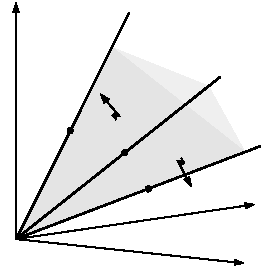
\includegraphics{part_1/chapter_2/figures/Figure3}};
	    \node (x0) at (0,-0.4) {$x_0$};
	    \node (x1) at (1.4,0.4) {$x_1$};
	    \node (x2) at (-1,-0.9) {$x_2$};
	    \node (a) at (-0.5,1.4) {$a$};
	    \node (S) at (-1.7,0.2) {$S$}; 
	\end{tikzpicture}
	\caption{The affine subspace $S$ generated by $x_0$ and $\nulls(a)$} \label{p1c2:fig:nill_space_a}		
\end{figure}


\section{Convex polyhedral set}

The feasible region of any linear programming problem is a convex polyhedral set, which we will simply refer to as a polyhedral set. That is because we are interested in polyhedral sets that are formed by an intersection of a finite number of half-spaces, and can thus only be convex (as we will see in a moment), creating redundancy in our context, but maybe some confusion overall. 

\subsection{Hyperplanes, half-spaces and polyhedral sets}

Definition \ref{p1c2:def:polyhedral_sets} formally states the structure we refer to as polyhedral sets.
%
\begin{definition}[Polyhedral set] \label{p1c2:def:polyhedral_sets}
	A polyhedral set is a set that can be described as
	$$
	S = \braces{x \in \reals^n : Ax \geq b},	
	$$
	where $A$ is an $m \times n$ matrix and $b$ is a $m$-vector.
\end{definition}
%
One important thing to notice is that polyhedral sets, as defined in Definition \ref{p1c2:def:polyhedral_sets}, as formed by the intersection multiple half-spaces. Specifically, let $\braces{a_i}_{i=1}^m$ be the rows of $A$. Then, the set $S$ can be described as 
%
\begin{equation}
	S = \braces{x \in \reals^n : a_i^\top x \geq b_i, i = 1,\dots, m}, 	
\end{equation}
%
which represents exactly the intersection of the half-spaces $a_i^\top x \geq b_i$. Furthermore, notice that the hyperplanes $a_i^\top x = b_i$, $\forall i \in \braces{1,\dots, m}$, are the boundaries of each hyperplane, and thus describe one of the faces of the polyhedral set, which is generally given by $\braces{x \in S : a_i^\top x \geq b_i}$ for a given face $i \in \braces{1,\dots, m}$. Figure \ref{p1c2:fig:hyperplanes_and_polyhedral_set} illustrates a hyperplane forming two half-spaces (also polyhedral sets) and how the intersection of five half-spaces form a (bounded) polyhedral set.

\begin{figure}[h]
			\begin{tikzpicture}
		    \node (pic) at (0,0) {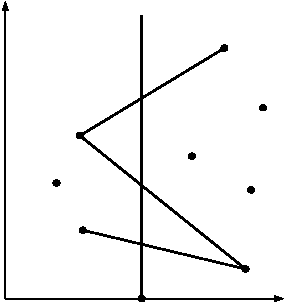
\includegraphics{part_1/chapter_2/figures/Figure4}};
		    \node (a) at (-4.5,0.2) {$a$};
			\node (ax=b) at (-3.6,-1.3) {$a^\top x =b$};
			\node (ax<b) at (-2.5, 0.8) {$a^\top x > b$};
			\node (ax>b) at (-2.3,-0.7) {$a^\top x < b$};
			\node (a1) at (1.5, -0.2) {$a_1$};
			\node (a2) at (2.8, 0.2) {$a_2$};
			\node (a3) at (1.8, 0.7) {$a_3$};
			\node (a4) at (2.9, -0.3) {$a_4$};
			\node (a5) at (2.2, -0.8) {$a_5$};
			\node[rotate = 90] (a1x=b1) at (0.1,0.2) {$a_1^\top x =b_1$};
			\node (a3x=b3) at (1.5,2.2) {$a_3^\top x =b_3$};
			\node (a2x=b2) at (4.5, 1) {$a_2^\top x =b_2$};
			\node (a4x=b4) at (4.4,-1.2) {$a_4^\top x =b_4$};
			\node (a5x=b5) at (1.3,-2) {$a_5^\top x =b_5$};
			\end{tikzpicture}
			\vspace{1pt}
		\caption{A hyperplane and its respective halfspaces (left) and the polyhedral set $\braces{x\in \reals^{2} : a_i^x \leq b_i, i =1,\dots, 5}$ (right).} \label{p1c2:fig:hyperplanes_and_polyhedral_set}		
	\end{figure}

You might finds authors referring to bounded polyhedral sets as polytopes, though this is not used consistently across references, sometimes with switched meanings (for example, using polytope to refer to a set defined as in Definition \ref{p1c2:def:polyhedral_sets} and using polyhedron to refer to a bounded version of $S$). In this text, we will only use the term polyhedral set to refer to sets defined as in Definition \ref{p1c2:def:polyhedral_sets} and use the term bounded whenever applicable.

% TODO: include a more rigorous presentation of face and facets. 


\subsection{Convexity of polyhedral sets}

As will see in more details in Part 2 of this text, convexity plays a crucial role in optimisation, being the ``watershed'' between easy and hard optimisation problems. One of the main reasons why we can solve challenging linear programming problems is due to the inherent convexity of polyhedral sets.

Let us first define the notion of convexity for sets, which is stated in Definition \ref{p1c2:def:convex_set} 

\begin{definition}[Convex set]\label{p1c2:def:convex_set} 
	A set $S \subseteq \reals^n$ is convex if, for any $x_1,x_2 \in S$ and any $\lambda \in [0,1]$, we have that $\overline{x} = \lambda x_1 + (1-\lambda) x_2 \in S$.
\end{definition}

Definition \ref{p1c2:def:convex_set} leads to a simple geometrical intuition: for a set to be convex, the line segment connecting any two points within the set must lie within the set. This is illustrated in Figure \ref{p1c2:fig:convex_sets}.

\begin{figure}
	\begin{tikzpicture}
		\node (pic) at (0,0) {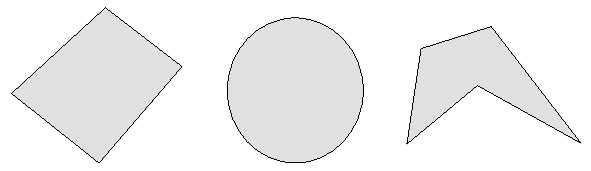
\includegraphics{part_1/chapter_2/figures/Figure5}};
		% Left pic line
		\node[circle, fill, minimum size=3pt, inner sep = 0pt] (x1) at (-4,-0.5) {};
		\node[above left] at (-4,-0.5) {$x_1$};
		\node[circle, fill, minimum size=3pt, inner sep = 0pt] (x2) at (-2.8,0.5) {};
		\node[above left] at (-2.8,0.5) {$x_2$};
		\draw[thick] (x1) -- (x2);
		% Center pic line
		\node[circle, fill, minimum size=3pt, inner sep = 0pt] (x1) at (-0.5,-0.5) {};
		\node[above left] at (-0.5,-0.5) {$x_1$};
		\node[circle, fill, minimum size=3pt, inner sep = 0pt] (x2) at (0.5,0.5) {};
		\node[above left] at (0.5,0.5) {$x_2$};
		\draw[thick] (x1) -- (x2);
		\node[circle, fill, minimum size=3pt, inner sep = 0pt] (x1) at (2.3, -0.3) {};
		\node[above] at (2.3, -0.3) {$x_1$};
		\node[circle, fill, minimum size=3pt, inner sep = 0pt] (x2) at (4,-0.3) {};
		\node[above left] at (4,-0.3) {$x_2$};
		\draw[thick] (x1) -- (x2);
	\end{tikzpicture}
	\caption{Two convex sets (left and middle) and one nonconvex set (right)} \label{p1c2:fig:convex_sets}
\end{figure}

Associated with the notion of convex sets are two important elements we will refer to later, when we discuss linear problems that embed \emph{integrality requirements}. The first is the notion of a convex combination, which is already contained in Definition \ref{p1c2:def:convex_set}, but can be generalised for an arbitrary number of points. The second consists of \emph{convex hulls}, which are sets formed by combining the convex combinations of all elements within a given set. As one might suspect, convex hulls are always convex sets, regardless whether the original set from which the points are drawn from is convex or not. These are formalised in Definition \ref{p1c2:def:convex_combination_hull} and illustrated in Figure \ref{p1c2:fig:convex_hulls}.

\begin{definition}[Convex combinations and convex hulls] \label{p1c2:def:convex_combination_hull}
	Let $x_1, \dots, x_k \in \reals^n$ and $\lambda_1,\dots, \lambda_k \in \reals$ such that $\lambda_i \geq 0$ for $i = 1, \dots, k$ and $\sum_{i=1}^k \lambda_i = 1$. Then
	\begin{enumerate}
		\item $x = \sum_{i=1}^k \lambda_i x_i$ is a \emph{convex combination} of $\braces{x_i}_{i=1}^k \in \reals^n$.
		\item The \emph{convex hull} of $\braces{x_i}_{i=1}^k \in \reals^n$, denoted $\conv(x_1, \dots, x_k)$, is the set of all convex combinations of $\braces{x_i}_{i=1}^k \in \reals^n$.
	\end{enumerate}		
\end{definition}

\begin{figure}
	\begin{tikzpicture}
		\node (pic) at (0,0) {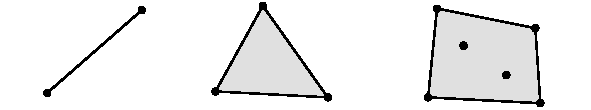
\includegraphics{part_1/chapter_2/figures/Figure6}};
		\node (x1l) at (-4.5,-0.7) {$x_1$};
		\node (x2l) at (-2.3, 0.7) {$x_2$};
		\node (x1c) at (-0.5, 1.1) {$x_1$};
		\node (x2c) at (0.8, -1) {$x_2$};
		\node (x3c) at (-1.5, -0.9) {$x_3$};
		\node (x1r) at (2.1, 1) {$x_1$};
		\node (x2r) at (4.4, 0.6) {$x_2$};
		\node (x3r) at (4.5, -0.9) {$x_3$};
		\node (x4r) at (1.9, -0.9) {$x_4$};
		\node (x5r) at (2.7, 0.4) {$x_5$};
		\node (x6r) at (3.8, -0.15) {$x_6$};
	\end{tikzpicture}
	\vspace{-6pt}
	\caption{The convex hull of two points is the line segment connecting them (left); The convex hull of three (centre) and six (right) points in $\reals^2$} \label{p1c2:fig:convex_hulls}
\end{figure}	

We are now ready to state the result that guarantees the convexity of polyhedral sets of the form
$$
	S = \braces{x \in \reals^n : Ax \le b}.
$$


\begin{theorem}[Convexity of polyhedral sets] \label{p1c2:thm:convexity}
	The following statements are true:
	\begin{enumerate}
		\item The intersection of convex sets is convex
		\item Every polyhedral set is a convex set
		\item A convex combination of a finite number of elements of a convex set also belongs to that set
		\item The convex hull of a finite number of elements is a convex set.			
	\end{enumerate}
\end{theorem}

\begin{proof}
	We provide proofs to each of the statements individually. 
	\begin{enumerate}
	 \item Let 	$S_i$, for $i \in I$, be convex sets and suppose that $x, y \in \bigcap_{i \in I} S_i$. Let $\lambda \in [0,1]$. Since $S_i$ are convex and $x,y \in S_i$ for all $i \in I$, $\lambda x + (1-\lambda) y \in S_i$ for all $i \in I$ and, thus, $\lambda x + (1-\lambda) y \in \bigcap_{i \in I} S_i$.
	
	\item Let $a \in \reals^n$ and $b \in \reals$. Let $x,y \in \reals^n$, such that $a^\top x \geq b$ and $a^\top y \geq b$. Let $\lambda \in [0,1]$. Then $a^\top (\lambda x + (1-\lambda)y) \geq \lambda b + (1-\lambda)b = b$, showing that half-spaces are convex. The result follows from combining this with (1).    
	
	\item By induction. Let $S$ be a convex set and assume that the convex combination of $x_1, \dots, x_k \in S$ also belongs to $S$. Consider $k+1$ elements $x_1, \dots, x_{k+1} \in S$ and $\lambda_1, \dots, \lambda_{k+1}$ with $\lambda_i \in [0,1]$ for $i = 1,\dots, k+1$ and $\sum_{i=1}^{k+1}\lambda_i = 1$ and $\lambda_{k+1} \neq 1$ (without loss of generality). Then

	\begin{equation}
		\sum_{i=1}^{k+1}\lambda_i x_i = \lambda_{k+1}x_{k+1} + (1 - \lambda_{k+1}) \sum_{i=1}^k \frac{\lambda_i}{1 - \lambda_{k+1}}x_i. \label{p1c2:eq:induction}
	\end{equation}								

		Notice that $\sum_{i=1}^{k}\frac{\lambda_i}{1 - \lambda_{k+1}} = 1$. Thus, using the induction hypothesis, $\sum_{i=1}^{k}\frac{\lambda_i}{1 - \lambda_{k+1}}x_i \in S$. Considering that $S$ is convex and using \eqref{p1c2:eq:induction}, we conclude that $\sum_{i=1}^{k+1}\lambda_{k+1}x_{k+1} \in S$, completing the induction.
		
	\item Let $S = \conv(x_1, \dots, x_k)$. Let $y = \sum_{i=1}^k \alpha_i x_i$ and $z = \sum_{i=1}^k \beta_ix_i$ be such that $y,z \in S$, $\alpha_i,\beta_i \geq 0$, and $\sum_{i=1}^k \alpha_i = \sum_{i=1}^k \beta_i = 1$. Let $\lambda \in [0,1]$. Then
		%
		\begin{equation}
			\lambda y + (1- \lambda)z = \lambda\sum_{i=1}^k \alpha_i x_i + (1-\lambda)\sum_{i=1}^k \beta_i x_i = \sum_{i=1}^k (\lambda \alpha_i + (1-\lambda) \beta_i)x_i. 	
		\end{equation}
		%
		Since $\sum_{i=1}^k \lambda \alpha_i + (1-\lambda) \beta_i = 1$ and $\lambda \alpha_i + (1-\lambda) \beta_i \geq 0$ for $i=1,\dots,k$, $\lambda y + (1- \lambda)z$ is a convex combination of $x_1, \dots, x_k$ and, thus, $\lambda y + (1- \lambda)z \in S$, showing the convexity of $S$. \qedhere	
	\end{enumerate}	
\end{proof}

Figure \ref{p1c2:fig:convexity_theorem_examples} illustrates some of the statements represented in the proof. For example, the intersection of the convex sets is always a convex set. One should notice however that the same does not apply to the union of convex sets. Notice that statement 2 proves that polyhedral sets as defined according to Definition \ref{p1c2:def:polyhedral_sets} are convex. Finally the third figure on the right illustrates the convex hull of four points as a convex polyhedral set containing the lines connecting any two points within the set. 
 
\begin{figure}
	\begin{tikzpicture}
%			\draw[help lines] (-5,-1) grid (5,1);
		\node (pic) at (0,0) {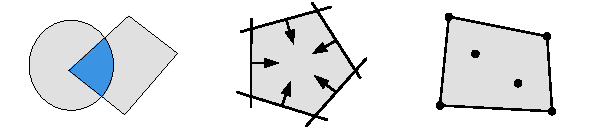
\includegraphics{part_1/chapter_2/figures/Figure7}};
	\end{tikzpicture}
    \vspace{-6pt}
	\caption{Illustration of statement 1 (left), 2 (centre), and 3 and 4 (right)} \label{p1c2:fig:convexity_theorem_examples}
\end{figure}	

We will halt our discussion about convexity for now and return to it in deeper details in Part 2. As it will become clearer then, the presence of convexity (which is a given in the context of linear programming, as we have just seen) is what allows us to conclude that the solutions returned by our optimisation algorithms are indeed optimal for the problem at hand. 


\section{Extreme points, vertices, and basic feasible solutions}

Now we focus on the algebraic representation of the most relevant geometric elements in the optimisation of linear programming problems. As we have seen in the graphical example in the previous chapter, the optimum of linear programming problems is generally located at the vertices of the feasible set. Furthermore, such vertices are formed by the intersection of $n$ constraints (in $n$-dimensional space, which comprises constraints that are active (or satisfied at the boundary of the half-space of said constraints).

First, let us formally define the notions of vertex and extreme point. Though in general these can refer to different objects, we will see that in the case of linear programming problems, if a point is a vertex, then it is an extreme point as well, being the converse also true.

\begin{definition}[Vertex] \label{p1c2:def:vertex}
	Let $P$ be a convex polyhedral set. The vector $x \in P$ is a vertex of $P$ if there exists some $c$ such that $c^\top x < c^\top y$ for all $y \in P$ with $y \neq x$.
\end{definition}

\begin{definition}[Extreme points]\label{p1c2:def:extreme_point}
	Let $P$ be a convex polyhedral set. The vector $x \in P$ is an extreme point of $P$ if there are no two vectors $y,z \in P$ (different than $x$) such that $x = \lambda y + (1 - \lambda)z$, for any $\lambda \in [0,1]$.
\end{definition}

Figure \ref{p1c2:fig:vertex_and_extreme_point} provides an illustration of the Definitions \ref{p1c2:def:vertex} and \ref{p1c2:def:extreme_point}. Notice that, while the definition of a vertex involves an additional hyperplane that, once placed on a vertex point, strictly contains the whole polyhedral set in one of the half-spaces it defines, with the exception of the vertex itself. On the other hand, the definition of an extreme point only relies on convex combinations of elements in the set itself. 

\begin{figure}
	\begin{tikzpicture}
		\node (pic) at (0,0) {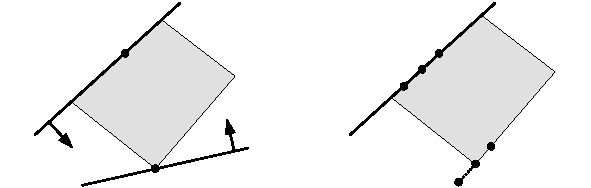
\includegraphics{part_1/chapter_2/figures/Figure8}};
		\node (Pl) at (-2.5, 0) {$P$};
		\node (Pr) at (3, 0) {$P$};
		\node (wl) at (-3, 0.9) {$w$};
		\node (xl) at (-2.3, -1.5) {$x$};
		\node (c1) at (-4, -1) {$c$};
		\node (c2) at (-0.9, -0.5) {$c$};
		\node[left] (cw) at (-2.3, 1.5) {$\braces{y : c^\top y = c^\top w}$};
		\node[right] (cx) at (-1.7, -1.4) {$\braces{y : c^\top y = c^\top x}$};
		\node (wr) at (2.1, 0.7) {$w$};
		\node (vr) at (2.4, 0.9) {$v$};
		\node (ur) at (1.8, 0.4) {$u$};
		\node (xr) at (3.1, -1.5) {$x$};
		\node (yr) at (3.4, -1.2) {$y$};
		\node (zr) at (2.8, -1.8) {$z$};
	\end{tikzpicture}
	\caption{Representation of a vertex (left) and a extreme point (right)} \label{p1c2:fig:vertex_and_extreme_point}
\end{figure}	

Now we focus on the description of active constraints under an algebraic standpoint. For that, let us first generalise our setting by considering all possible types of linear constraints. That is, let us consider the convex polyhedral set $P \subset \reals^n$, formed by the set of inequalities and equalities:
%
\begin{align*}
	& a_i^\top x \geq b, i \in M_1, \\ 
	& a_i^\top x \leq b, i \in M_2, \\
	& a_i^\top x = b, i \in M_3.
\end{align*}

Definition \ref{p1c2:fig:active_constraint} formalises the notion of active constraints. This is illustrated in Figure \ref{p1c2:fig:active_constraints}, where the polyhedral set $P = \braces{x \in \reals^3 : x_1 + x_2 + x_3 = 1, x_i \geq 0, i =1,2,3}$ is represented. Notice that, while points $A$, $B$, $C$ and $D$ have 3 active constraints, $E$ only has 2 active constraints ($x_2 = 0$ and $x_1 + x_2 + x_3 = 1$).

\begin{definition}[Active (or binding) constraints] \label{p1c2:fig:active_constraint}
	If a vector $\overline{x}$ satisfies $a_i^\top \overline{x} = b_i$ for some $i \in M_1, M_2$, or $M_3$, we say that the corresponding constraints are active (or binding).
\end{definition}

\begin{figure}[h]
	\begin{tikzpicture}
		\node (pic) at (0,0) {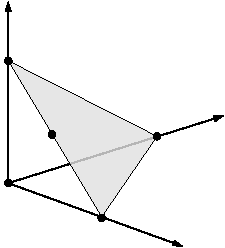
\includegraphics{part_1/chapter_2/figures/Figure9}};
		\node (x1) at (1.5, -2) {$x_1$};
		\node (x2) at (1.7, 0.4) {$x_2$};
		\node (x3) at (-2.1, 2) {$x_3$};
		\node (P) at (0, -0.5) {$P$};
		\node[left] (A) at (-1.1, 1.3) {$A$};
		\node[left] (B) at (-1.8, -1) {$B$};
		\node[right] (C) at (-0.5, -1.9) {$C$};
		\node[above] (D) at (0.9, -0.1) {$D$};
		\node[right] (E) at (-1.6, -0.2) {$E$};
	\end{tikzpicture}
	\caption{Representation of $P$ in $\reals^3$.} \label{p1c2:fig:active_constraints}
\end{figure}	


Theorem \ref{p1c2:thm:active_const} sows a thread between having a collection of active constraints forming a vertex and being able to describe it as a basis of a subspace that is formed by the vectors $a_i$ that form these constraints. This link is what will allow us to characterise vertices by their forming active constraints.

\begin{theorem}[Properties of active constraints]\label{p1c2:thm:active_const}
	Let $\overline{x} \in \reals^n$ and $I = \braces{ i \in M_1 \cup M_2 \cup M_3 \mid a_i^\top \overline{x} = b_i}$. Then, the following are equivalent:
	\begin{enumerate}
		\item There exists $n$ vectors in $\braces{a_i}_{i \in I}$ that are linearly independent.  
		\item The $\spans(\braces{a_i}_{i \in I})$ spans $\reals^n$. That is, every $x \in \reals^n$ can be expressed as a linear combination of $\braces{a_i}_{i \in I}$.
		\item The system of equations $\braces{a_i ^\top x = b_i}_{i \in I}$ has a unique solution.
	\end{enumerate}
\end{theorem}

\begin{proof}
	Suppose that $\braces{a_i}_{i \in I}$ spans $\reals^n$, implying that the $\spans(\braces{a_i}_{i \in I})$ has dimension $n$. By Theorem \ref{p1c2:thm:LI_and_bases} (part 1), $n$ of these vectors form a basis for $\reals^n$ and are, thus, linearly independent. Moreover, they must span $\reals^n$ and therefore every $x \in \reals^n$ can be expressed as a combination of $\braces{a_i}_{i \in I}$. This connects (1) and (2).
	
	Assume that the system of equations $\braces{a_i ^\top x = b_i}_{i \in I}$ has multiple solutions, say $x_1$ and $x_2$. Then, the nonzero vector $d = x_1 - x_2$ satisfies $a_i^\top d = 0$ for all $i \in I$. As $d$ is orthogonal to every $a_i$, $i \in I$, $d$ cannot be expressed as a combination of $\braces{a_i}_{i \in I}$ and, thus, $\braces{a_i}_{i \in I}$ do not span $\reals^n$.
	
	Conversely, if $\braces{a_i}_{i \in I}$ do not span $\reals^n$, choose $d \in \reals^n$ that is orthogonal to $\spans(\braces{a_i}_{i \in I})$. If $x$ satisfies $\braces{a_i ^\top x = b_i}_{i \in I}$, so does $\braces{a_i ^\top (x + d) = b_i}_{i \in I}$, thus yielding multiple solutions. This connects (2) and (3). \qedhere
\end{proof}

Notice that Theorem \ref{p1c2:thm:active_const} implies that there are (at least) \emph{$n$ active constraints ($a_i$)} that are \emph{linearly independent} at $\overline{x}$. This is the reason why we will refer to $\overline{x}$ and any vertex forming solution a \emph{basic solution}, of which we will be interested in those that are feasible, i.e., that satisfy all constraints $i \in M_1 \cup M_2 \cup M_3$. Definition \ref{p1c2:def:basic_feasible_solution} provides a formal definition of these concepts.

\begin{definition}[Basic feasible solution (BFS)] \label{p1c2:def:basic_feasible_solution}
	Consider a convex polyhedral set $P \subset \reals^n$ defined by linear equality and inequality constraints, and let $\overline{x} \in \reals^n$.
	\begin{enumerate}
		\item $\overline{x}$ is a \emph{basic solution} if 
		\begin{enumerate}
			\item All equality constraints are active and,
			\item Out of the constraints active at $\overline{x}$, $n$ of them are linearly independent.
		\end{enumerate}
		\item if $\overline{x}$  is a basic solution satisfying all constraints, we say $\overline{x}$ is a basic feasible solution. 
	\end{enumerate}
\end{definition}

Figure \ref{p1c2:fig:BFS} provides an illustration of the notion of basic solutions, and show how only a subset of the basic solutions are feasible. As one might infer, these will be the points of interest in out future developments, as these are the candidates for optimal solution.

\begin{figure}[h]
	\begin{tikzpicture}
		\node (pic) at (0,0) {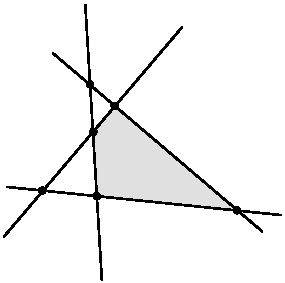
\includegraphics{part_1/chapter_2/figures/Figure10}};
		\node[above] (A) at (-0.7, 1) {$A$};
		\node[left] (B) at (-0.9, 0.2) {$B$};
		\node[right] (C) at (-0.4, 0.7) {$C$};
		\node[below] (D) at (1.6, -1.2) {$D$};
		\node[below] (E) at (-0.5, -1) {$E$};
		\node[above] (F) at (-1.8, -0.8) {$F$};
		\node (P) at (-0.3, -0.3) {$P$};
	\end{tikzpicture}
	\caption{Points $A$ to $F$ are basic solutions; $B$,$C$,$D$, and $E$ are BFS.} \label{p1c2:fig:BFS}
\end{figure}		

We finalise stating the main result of this chapter, which formally confirms the intuition we developed so far. That is, for convex polyhedral sets, the notion of vertices and extreme points coincide and these points can be represented as basic feasible solutions. This is precisely the link that allows to treat the feasible region of linear programming problems under a purely algebraic characterisation of the candidates for optimal solutions, those described uniquely by a subset of constraints of the problem.

\begin{theorem}[BFS, extreme points and vertices]\label{p1c2:thm:BFS_vertex_extreme_point}
	Let $P \subset \reals^n$ be a convex polyhedral set and let $\overline{x} \in P$. Then, the following are equivalent
	$$	\overline{x} \text{ is a vertex} \iff \overline{x} \text{ is an extreme point} \iff \overline{x} \text{ is a BFS}.	
	$$
\end{theorem}


\begin{proof}
	Let $P =\{ x \in \reals^n \mid a_i^\top x \geq b_i, i \in M_1, a_i^\top x = b_i, i \in M_2\}$, and $I = \braces{i \in M_1 \cup M_2 \mid a_i^\top x = b_i}$.
	
	\begin{enumerate}
		\item (Vertex $\Rightarrow$ Extreme point) Suppose $\overline{x}$ is a vertex. Then, there exists some $c \in \reals^n$ such that $c^\top\overline{x} < c^\top x$, for every $x \in P$ with $x \neq \overline{x}$ (cf. Definition \ref{p1c2:def:vertex}). Take $y,z \in P$ with $y,z \neq \overline{x}$. Thus $c^\top\overline{x} < c^\top y$ and $c^\top\overline{x} < c^\top z$. For $\lambda \in [0,1]$, $c^\top \overline{x} < c^\top(\lambda y + (1-\lambda)z)$ implying that $\overline{x} \neq \lambda y + (1-\lambda)z$, and is thus an extreme point (cf. Definition \ref{p1c2:def:extreme_point}).
		
		\item (Extreme point $\Rightarrow$ BFS) suppose $\overline{x} \in P$ is not a BFS. Then, there are no $n$ linearly independent vectors within $\braces{a_i}_{i \in I}$. Thus $\braces{a_i}_{i \in I}$ lie in a proper subspace of $\reals^n$. Let the nonzero vector $d \in \reals^n$ be such that $a_i^\top d = 0$, for all $i \in I$.
			
			Let $\epsilon > 0$, $y = \overline{x} + \epsilon d$, and $z = \overline{x} - \epsilon d$. Notice that $a_i^\top y = a_i^\top z = b_i$, for all $i \in I$. Moreover, for $i \neq I$, $a_i^\top x > b$ and, provided that $\epsilon$ is sufficiently small (such that $\epsilon|a_i^\top d| < a_i ^\top \overline{x} - b_i $), we have that $a_i ^\top x \geq b_i$. Thus $y \in P$, and by a similar argument, $z \in P$. Now, by noticing that $\overline{x} = \frac{1}{2}y + \frac{1}{2}z$, we see that $\overline{x}$ is not an extreme point. 			 
		\item (BFS $\Rightarrow$ Vertex) Let $\overline{x}$ be a BFS. Define $c = \sum_{i \in I} a_i$. Then
			\begin{equation*}
				c^\top \overline{x} = \linebreak \sum_{i \in I} a_i^\top \overline{x} = \sum_{i \in I} b_i.	 			 	
	 		\end{equation*}
			Also, for any $x \in P$, we have that 
			\begin{equation*}
				c^\top x = \sum_{i \in I} a_i^\top x \geq \sum_{i \in I} b_i, 	 	
	 		\end{equation*}
	 		since $a_i^\top x \geq b_i$ for $i \in M_1 \cup M_2$. Thus, for any $x \in P$, $c^\top \overline{x} \leq c^\top x$, making $\overline{x}$ a vertex (cf. Definition \ref{p1c2:def:vertex}). \qedhere
	\end{enumerate} 	
\end{proof}

Some interesting insights emerge from the proof of Theorem \ref{p1c2:thm:BFS_vertex_extreme_point}, upon which we will build our next developments. First, notice how the definition of vertex encodes a concept of optimality, since it implies that $\overline{x}$ is a unique minimiser (i.e., all other feasible points $y$ are such that $c^\top\overline{x} < c^\top y$). Also, once the relationship between being a vertex/ extreme point and a BFS is made, it means that $\overline{x}$ can be recovered as the unique solution of a system of linear equations, these equations being the active constraints at that vertex. This means that the list of all candidate points for optimal solution can be obtained by simply looking at all possible combinations of $n$ active constraints, discarding those that are infeasible. This means that the number of candidates for optimal solution is \emph{finite} and can be bounded by $\binom{m}{n}$, where $m=| M_1 \cup M_2 |$. 


\section{Exercises}

\subsection*{Exercise 2.1: Polyhedral sets}
Which of the following sets are polyhedral?
\begin{itemize}
\item[(a)] $\{(x,y)\in\mathbb{R}^2~|~ x \cos \theta + y\sin\theta \leq 1,\theta\in[0,\pi/2],x\geq0,y\geq0\}$
\item[(b)] $\{x\in\mathbb{R}~|~ x^2-8x+15\leq 0\}$
\item[(c)] The empty set ($\emptyset$).
\end{itemize}

\subsection*{Exercise 2.2: Convexity of polyhedral sets}
Prove the following theorem.

\begin{theorem*}[Convexity of polyhedral sets] 
	%	\vspace{-3pt}
	\emph{The following convexity properties about convex sets can be said:}
	\begin{enumerate}
		\item The intersection of convex sets is convex
		\item Every polyhedral set is a convex set
		\item A convex combination of a finite number of elements of a convex set is also belongs to that set
		\item The convex hull of a finite number of elements is a convex set.			
	\end{enumerate}
\end{theorem*}

Note: the theorem is proved in the notes. Use this as an opportunity to revisit the proof carefully, and try to take as many steps without consulting the text as you can. This is a great exercise to help you internalise the proof and its importance in the context of the material. I strongly advise against blindly memorising it, as I suspect you will never (in my courses, at least) be requested to recite the proof literally.


\subsection*{Exercise 2.3: Properties of active constraints}
Let us consider the convex polyhedral set $P \subset \reals^n$, formed by the set of equalities and inequalities:
%
\begin{align*}
	a_i^\top x \geq b, i \in M_1, \\
	a_i^\top x \leq b, i \in M_2, \\
	a_i^\top x = b, i \in M_3.
\end{align*}
%

Prove the following result.

\begin{theorem*}[Properties of active constraints]
	Let $\overline{x} \in \reals^n$ and $I = \braces{ i \in M_1 \cup M_2 \cup M_3 \mid a_i^\top \overline{x} = b_i}$. Then, the following are equivalent:
	\begin{enumerate}
		\item There exists $n$ vectors in $\braces{a_i}_{i \in I}$ that are linearly independent.  
		\item The $\spans(\braces{a_i}_{i \in I})$ spans $\reals^n$. That is, every $x \in \reals^n$ can be expressed as a combination of $\braces{a_i}_{i \in I}$.
		\item The system of equations $\braces{a_i ^\top x = b_i}_{i \in I}$ has a unique solution.
	\end{enumerate}
\end{theorem*}

Note: see Exercise 2.2.

\subsection*{Exercise 2.4: Vertex, extreme points, and BFSs}
Prove the following result.

\begin{theorem*}[BFS, extreme points and vertices]
	Let $P \subset \reals^n$ be a convex polyhedral set and let $\overline{x} \in P$. Then, the following are equivalent
	\begin{enumerate}
		\item $\overline{x}$ is a vertex;
		\item $\overline{x}$ is a extreme point;
		\item $\overline{x}$ is a BFS;	
	\end{enumerate}
\end{theorem*}

Note: see Exercise 2.2.

\subsection*{Exercise 2.5: Binding constraints applications} 
Given the linear program defined by the system of inequalities below,

\begin{center}
	\begin{enumerate}
		\begin{tabular}{*4c}
			$\max$ & $2x_1 + x_2$ & \\
			s.t. \\
			& $2x_1 + 2x_2$ & $\leq$ & $9$  \\
			& $2x_1 -  x_2$ & $\leq$ & $3$  \\
			& $ x_1 -  x_2$ & $\leq$ & $1$  \\
			& $x_1$         & $\leq$ & $2.5$\\
			& $x_2$         & $\leq$ & $4$  \\
			\\
			\multicolumn{4}{c}{$x_1, x_2 \geq 0$}\\
		\end{tabular}
	\end{enumerate}
\end{center}

\noindent assess the following points relative to the polyhedron defined in $\reals^2$ by this system and classify them as in $(i)$ belonging to which active constraint(s), $(ii)$ being a non-feasible/basic/basic feasible solution, and $(iii)$ being an extreme point, vertex, or outside the polyhedron. Use Theorem \ref{p1c2:thm:active_const} and Theorem \ref{p1c2:thm:BFS_vertex_extreme_point} to check if your classification is correct.

\begin{itemize}
	\item[(a)] $(1.5,0)$
	\item[(b)] $(1,0)$
	\item[(c)] $(2,1)$
	\item[(d)] $(1.5,3)$
\end{itemize}

 


	

		
	
	\part{Adaptive Linear Optimization} \label{part_2}
		
	\chapter{Introduction}
	\section{What is optimisation?}

An optimisation is one of these words that has many meanings, depending on the context you take as a reference. In the context of this course, optimisation refers to \emph{mathematical optimisation}, which is a discipline of applied mathematics.

In mathematical optimisation, we build upon concepts and techniques from calculus, analysis, linear algebra, and other domains of mathematics to develop methods that allow us finding values for variables within a given domain that maximise (or minimise) the value of a function. In specific, we are trying to solve the following general problem:
%
\begin{align}
    \min &f(x) \label{eq:opt_prob} \\
    \text{s.t.}   &x \in X. \nonumber
\end{align}
%
%where $x \in \reals^n$ is a vector of $n$ \emph{variables}, $f:\mathbb{R}^n \mapsto \reals$ is a \emph{function} to be optimised (minimised) and $X \subseteq \reals^n$ is a \emph{domain} containing acceptable values for $x$.

In a general sense, these problems can be solved by employing the following strategy:
%
\begin{enumerate}
    \item Analysing properties of functions under specific domains and deriving the conditions that must be satisfied such that a point $x$ is a candidate optimal point.
    \item Applying numerical methods that iteratively searches for points satisfying these conditions. 
\end{enumerate}
%
This idea is central in several domains of knowledge, and very often are defined under area-specific nomenclature. Fields such as economics, engineering, statistics, machine learning and, perhaps more broadly, operations research, are intensive users and developers of optimisation theory and applications. 

\subsection{Mathematical programming and optimisation}

Operations research and mathematical optimisation are somewhat intertwined, as they both were born around a similar circumstance. %(Include something on the history of OR)

I like to separate \emph{mathematical programming} from (mathematical) \emph{optimisation}. Mathematical programming is a modelling paradigm, in which we rely on (very powerful, I might add) analogies to model \emph{real-world} problems. In that, we look at a given decision problem considering that
%
\begin{itemize}
    \item \emph{variables} represent \emph{decisions}, as in a business decision or a course of action. Examples include setting the parameter of (e.g., prediction) model, production systems layouts, geometries of structures, topologies of networks, and so forth; 
    \item \emph{domain} represents business rules or \emph{constraints}, representing logic relations, design or engineering limitations, requirements, and such; 
    \item function is an \emph{objective function} that provides a measure of solution quality.  
\end{itemize}
%    
With these in mind, we can represent the decision problem as a \emph{mathematical programming model} of the form of \eqref{eq:opt_prob} that can be solved using \emph{optimisation} methods. From now on, we will refer to this specific class of models as mathematical optimisation models, or optimisation models for short. We will also use the term to \emph{solve the problem} to refer to the task of finding optimal solutions to optimisation models.

This course is mostly focused on the optimisation techniques employed to find optimal solutions for these models. As we will see, depending on the nature of the functions $f$ and $g$ that are used to formulate the model, some methods might be more or less appropriate. Further complicating the issue, for models of a given nature, there might be alternative algorithms that can be employed and with no generalised consense whether one method is generally better performing than another.

\subsection{Types of mathematical optimisation models}

In general, the simpler the assumptions on the parts forming the optimisation model, the more efficient are the methods to solve such problems. 

Let us define some additional notation that we will use from now on. Consider a model in the general form
%
\begin{align*}
	\mini & f(x) \\
	\st   & g_i(x) \leq 0, i = 1, \dots, m \\
	      & h_i(x) = 0, i = 1, \dots, l \\
	      & x \in X,  
\end{align*}
%
where $f: \reals^n \mapsto \reals$ is the objective function, $g:\reals^m \mapsto \reals^m$ is a collection of $m$ inequality constraints and $h: \reals^n \mapsto \reals^l$ is a collection of $l$ equality constraints.

{\bf Remark:} in fact, every inequality constraint can be represented by an equality constraint by making $h_i(x) = g_i(x) + x_{n+1}$ and augmenting the decision variable vector $x \in \reals^n$ to include the slack variable $x_{n+1}$. However, since these constraints are of very different nature, we will explicitly represent both whenever necessary.

The most general types of models are the following. We also use this as an opportunity to define some (admittedly confusing) nomenclature from the field of operations research that we will be using in these notes.
%
\begin{enumerate}
    \item \emph{Unconstrained models:} in these, the set $X = \reals^n$ and $m=l=0$. These are prominent in, e.g., machine learning and statistics applications, where $f$ represents a measure of model fitness or prediction error.  
    \item \emph{Linear programming (LP):} presumes linear objective function. $f(x) = c^\top x$ and constraints $g$ and $h$ affine, i.e., of the form $a_i^\top x - b_i$, with $a_i \in \reals^n$ and $b \in \reals$. Normally, $X = \braces{x \in \reals^n \mid x_j \geq 0, j = 1,\dots, n}$ enforce that decision variables are constrained to be the nonnegative orthant.
    \item \emph{Nonlinear programming (NLP):} some or all of the functions $f$, $g$, and $h$ are nonlinear.
    \item \emph{Mixed-integer (linear) programming (MIP):} consists of an LP in which some (or all) of the variables are constrained to be integers. In other words, $X \subseteq \reals^k \times \integers^{n-k}$. Very frequently, the integer variables are binary terms, i.e., $x_i \in \braces {0,1}$, for $i = 1,\dots, n-k$ and are meant to represent true-or-false or yes-or-no conditions.
    \item \emph{Mixed-integer nonlinear programming (MINLP):} are the intersection of MIPs and NLPs.  
\end{enumerate}

{\bf Remark:} notice that we use the vector notation $c^\top x = \sum_{j \in J} c_j x_j$, with $J = \braces{1,\dots,N}$. This is just a convenience for keeping the notation compact. 


\section{Examples of applications}


We now discuss a few examples to illustrate the nature of the problems to which we will develop solution methods and their applicability to real-world contexts. 

\subsection{Resource allocation and portfolio optimisation} \label{sec:resource_allocation}

In a general sense, any mathematical optimisation model is an instantiation of the \emph{resource allocation problem}. A resource allocation problem consists of how to design an optimal allocation of resources to tasks, such that a given outcome is optimised. 

Classical examples typically include production planning settings, in which raw materials or labour resources are inputted into a system and a collection of products, a production plan, results from this allocation. The objective is to find the best production plan, that is, a plan with the maximum profit or minimum cost. Resource allocation problems can also appear in a less obvious setting, where the resources can be the capacity of transmission lines in an energy generation planning setting, for example.

Let $i \in I = \braces{1,\dots, M}$ be a collection of resources and $j \in J = \braces{1,\dots,N}$ be a collection of products. Suppose that, to produce one unit of product $j$, a quantity $a_{ij}$ of resource $i$ is required. Assume that the total availability of resource $i$ is $b_i$ and that the return per unit of product $j$ is $c_j$.

Let $x_j$ be the decision variable representing total of product $j$ produced. The resource allocation problem can be modelled as
%
\begin{align}
	\maxi \ & \sum_{j \in J} c_j x_j \label{ex1:obj} \\
	\st & \sum_{j \in J}a_{ij} x_j \leq b_i, \ \forall i \in I \label{ex1:const1} \\
	& x_j \geq 0, \ \forall j \in J. \label{ex1:const2}
\end{align} 
%
Equation \eqref{ex1:obj} represents the objective function, in which we maximise the total return obtained from a given production plan. Equation \eqref{ex1:const1} quantify the resource requirements for a given production plan and enforce that such a requirement does not exceed the resource availability. Finally, constraint \eqref{ex1:const2} defines the domain of the decision variables.

Notice that, as posed, the resource allocation problem is linear. This is perhaps the most basic, and also most diffused setting for optimisation models for which very reliable and mature technology is available. In this course, we will concentrate on methods that can solve variants of this model in which the objective function and/or the constraints are required to include nonlinear terms. 

One classic variant of resource allocation that include nonlinear terms is the \emph{portfolio optimisation problem}. In this, we assume that a collection of assets $j \in J = \braces{1,\dots, N}$ are available for investment. In this case, capital is the single (actual) resource to be considered. Each asset has random return $R_j$, with an expected value $\mathbb{E}[R_j] = \mu_j$. Also, the covariance between two assets $i,j \in J$ is given by $\sigma_{ij} = \mathbb{E}[(R_i - \mu_i)(R_j - \mu_j)]$, which can be denoted as the covariance matrix 
%
\begin{align*}
	\Sigma = \begin{bmatrix}
		\sigma_{11} & \dots & \sigma_{1N} \\ 
		\vdots      & \ddots & \vdots \\
		\sigma_{N1}  & \dots & \sigma_{NN}
	\end{bmatrix}
\end{align*}
%
Markowitz (1952) proposed using $x^\top\Sigma x$ as a risk measure that captures the variability in the return of the assets. Given the above, the optimisation model that provides the investment portfolio with the least risk, given a minimum requirement $\epsilon$ in terms of expected returns is given by
%
\begin{align}
	\mini \ &  x^\top\Sigma x \label{ex2:obj} \\
	\st & \mu^\top x  \geq \epsilon \label{ex2:const1}\\
	& 0 \leq x_j \leq 1, \ \forall j \in J. \label{ex2:const2}
\end{align} 
%
Objective function \eqref{ex2:obj} represents the portfolio risk to be minimised, while constraint \eqref{ex2:const1} enforces that the expected return must be at least $\epsilon$. Notice that $\epsilon$ can be seen as a resource that has to be (at least) completely depleted, if one wants to do a parallel with the resource allocation structure discussed early. Constraint \eqref{ex2:const2} defined the domain of the decision variables. Notice how the problem is posed in a scaled form, where $x_j \in [0,1]$ represents a percentage of a hypothetical available capital for investment.

In this example, the problem is nonlinear due to the quadratic nature of the objective function $x^\top\Sigma x = \sum_{i,j \in J} \sigma_{ij}x_ix_j$. As we will see later on, there are efficient methods that can be employed to solve quadratic problems like this.


\subsection{The pooling problem: refinery operations planning}

The \emph{pooling problem} is another example of a resource allocation problem that naturally presents nonlinear constraints. In this case, the production depends on \emph{mixing operations}, known as pooling, to obtain certain product specification for a given property.

As an illustration, suppose that products $j \in J = \braces{1,\dots,N}$ are produced by mixing byproducts $i \in I_j \subseteq I = \braces{1,\dots,M}$. Assume that the qualities of byproducts $q_i$ are known and that there is no reaction between byproducts. Each product is required to have a property value $q_j$ within an acceptable range $[\underline{q}_j, \overline{q}_j]$ to be classified as product $j$. In this case, mass and property balances are calculated as
%
\begin{align}
	& x_j  = \sum_{i \in I_j}{x_i}, \ \forall j \in J \\
	& q_j = \frac{\sum_{i \in I_j}q_ix_i}{x_j}, \ \forall j \in J \label{ex3:const2}.
\end{align}
%
These can then incorporated into the resource allocation problem accordingly. One key aspect associated with pooling problem formulations is that the property balances represented by \eqref{ex3:const2} define \emph{nonconvex} feasibility regions. As we will see later, convexity is a powerful property that allows for developing efficient solution methods and its absence typically compromises computational performance and tractability in general.

  
\subsection{Robust optimisation}

Robust optimisation is a subarea of mathematical programming concerned with models that support decision-making under \emph{uncertainty}. In specific, the idea is to devise a formulation mechanism that can guarantee feasibility of the optimal solution in face of variability, ultimately taking a risk-averse standpoint. 

Consider the resource allocation problem from Section \ref{sec:resource_allocation}. Now, suppose that the parameters $\tilde{a}_i \in \reals^N $ associated with a given constraint $i \in I = \braces{1,\dots,M}$ are uncertain with a unknown probability distribution. The resource allocation problem can then be formulated as
%
\begin{align*}
	\maxi \ &  c^\top x  \\
	\st & \tilde{a}_{i}^\top x \leq b_i, \ \forall i \in I  \\
	& x_j \geq 0, \ \forall j \in J. 
\end{align*} 
%
Let us assume that the only information available are observations $\hat{a}_i$, from which we can estimate a nominal value $\overline{a}_i$. This is illustrated in Figure \ref{fig:random_observations}, in which 100 random observations are generated for $\tilde{a_i} = [\tilde{a}_{i1}, \tilde{a}_{i2}]$ with $\tilde{a}_{i1} \sim \text{Normal}(10,2)$ and $\tilde{a}_{i2} \sim \text{Normal}(5,3)$ for a single constraint $i \in I$. The nominal values are assumed to have coordinates given by the average values used in the Normal distributions. 
%
\begin{figure}[h]
	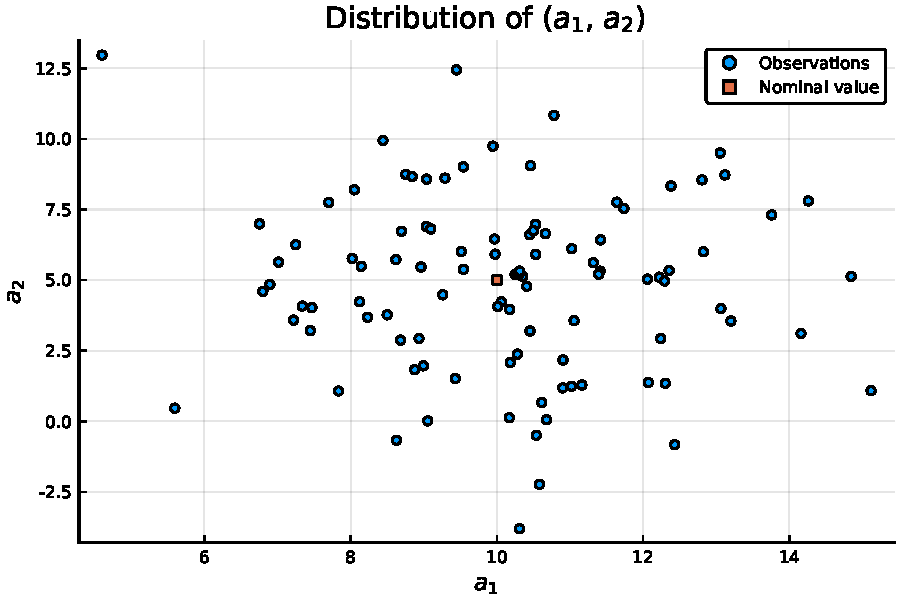
\includegraphics[width=0.8\textwidth]{part_2/chapter_1/figures/data_no_ellipsoid.pdf}
	\caption{One hundred random realisations for $\tilde{a}_i$.} \label{fig:random_observations}
\end{figure}
%
Our objective is to develop a model that incorporates a given level of protection in terms of feasibility guarantees. That is, we would like to develop a model that provides solutions that are guaranteed to remain feasible if the realisation of $\tilde{a}_i$ falls within an \emph{uncertainty set} $\epsilon_i$ of size controlled by the parameter $\Gamma_i$. The idea is that the bigger the uncertainty set $\epsilon_i$, the more robust is the solution, which typically comes at the expense of accepting solutions with expected worse performance.

The tractability of robust optimisation models depends on the geometry of the uncertainty set employed. Let us assume in what follows that 
%
\begin{align}
	\epsilon_i = \braces{\overline{a}_i + P_iu \mid ||u||_2 \leq \Gamma_i} \label{eq:ellipsoid}
\end{align}
%
is an ellipsoid with the characteristic matrix $P_i$ (i.e., its eigenvalues show how the ellipsoid extends in every direction from $\overline{a}_i$) and $\Gamma_i$ employs a scaling of the ellipsoid size.

{\bf Remark:} an alternative (perhaps more frequent) characterisation of an ellipsoid $\epsilon \subset \reals^n$ centred at $\overline{x}$ is given by $\epsilon = \braces{x \in \reals^n \mid (x - \overline{x})^\top A(x - \overline{x}) = 1}$. By making $A = P^{-2}$, we recover the representation in \eqref{eq:ellipsoid}.

We can now formulate the \emph{robust counterpart}, which consists of a risk-averse version of the original resource allocation problem. In that, we try to anticipate the worst possible outcome and make decisions that are both optimal and guarantee feasibility in this worst-case sense. This standpoint translates into the following optimisation model.
%
\begin{align}
	\maxi \ &  c^\top x \nonumber \\
	\st & \maxi_{a_{i} \in \epsilon_i}\braces{a_i^\top x} \leq b_i, \ \forall i \in I \label{ex3:robust_const}\\
	& x_j \geq 0, \forall j \in J. \nonumber
\end{align}
%
Notice how the constraint \eqref{ex3:robust_const} has an embedded optimisation problem, turning into a \emph{bi-level optimisation} problem. This highlights the issue associated with tractability, since solving the whole problem strongly depends on deriving tractable equivalent reformulations.

Assuming that the uncertainty set $\epsilon_i$ is an ellipsoid, the following result holds.
%
\begin{align}
	\max_{a_{i} \in \epsilon_i}\braces{a_i^\top x}  & = \overline{a}_i^\top x + \max_u\braces{u^\top P_i x : ||u||_2 \leq \Gamma_i} \label{eq:robust_set1}\\
	& = \overline{a}_i^\top x + \Gamma_i||P_i x||_2. \label{eq:robust_set2}
\end{align}
%
In \eqref{eq:robust_set1}, we recast the inner problem in terms of the ellipsoidal uncertainty set, ultimately meaning that we recast the inner maximisation problem in terms of variable $u$. Since the only constraint is $||u||_2 \leq \Gamma_i$, in \eqref{eq:robust_set2} we can derive a closed form for the inner optimisation problem.

With the closed form derived in \eqref{eq:robust_set2}, we can reformulate the original bi-level problem as a tractable single-level problem of the following form
%
\begin{align}
	\maxi \ &  c^\top x \nonumber \\
	\st & \overline{a}_i^\top x + \Gamma_i||P_i x||_2 \leq b_i, \ \forall i \in I \label{eq:robust_counter1}\\
	& x_j \geq 0, \ \forall j \in J. \nonumber
\end{align} 
%
Notice how the term $\Gamma_i||P_i^\top x||_2$ creates a buffer for constraint \eqref{eq:robust_counter1}, ultimately preventing the complete depletion of the resource. Clearly, this will lead to a suboptimal solution when compared to the original deterministic at the expense of providing protection against deviations in coefficients $a_i$. This difference is often referred to as the \emph{price of robustness}.

In Figure \ref{fig:ellipsoids}, we show the ellipsoidal sets for two levels of $\Gamma_i$ for a single constraint $i$. We define 
%
\begin{align}
	\epsilon_i = \braces{\begin{bmatrix} 10 \\ 5 \end{bmatrix} + \begin{bmatrix} 2 & 0 \\ 0 & 3 \end{bmatrix} \begin{bmatrix} u_1 \\ u_2 \end{bmatrix}}
\end{align}
%
using the average and standard deviation of the original distributions that generated the observations. We plot the ellipsoids for $\Gamma_1 = 1$ and $\Gamma_2 = 1.5$, illustrating how the protection level increases as $\Gamma$ increases. This can be inferred since the uncertainty set covers more of the observations and the formulation is such that feasibility is guaranteed for any observation within the uncertainty set. 
%
\begin{figure}
	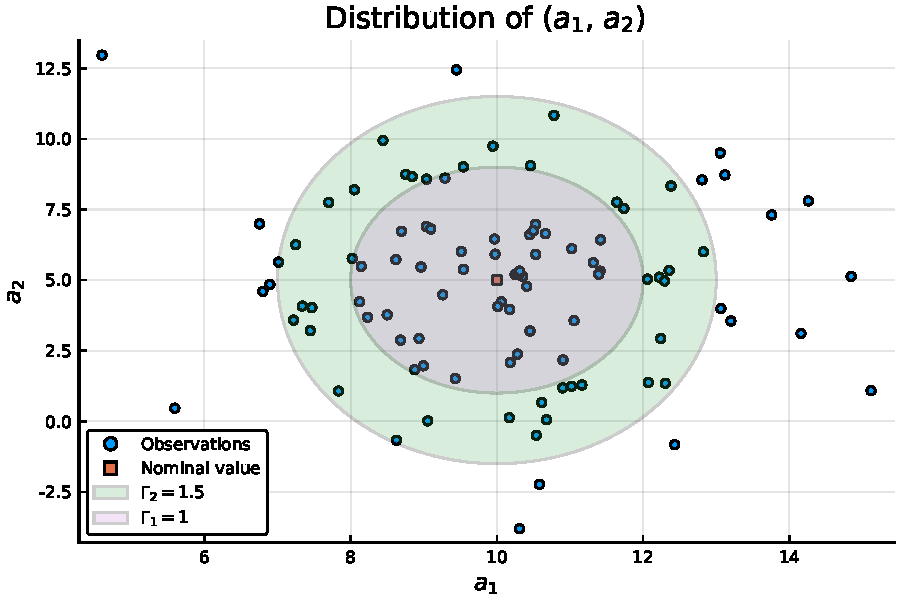
\includegraphics[width=0.8\textwidth]{part_2/chapter_1/figures/data_with_ellipsoid.pdf}
	\caption{One hundred random realisations for $\tilde{a}_i$.} \label{fig:ellipsoids}
\end{figure}
%


\subsection{Classification: support-vector machines}

This is an example in which the resource allocation structure within the optimisation model is not as obvious. Suppose we are given a data set $D \in \reals^{n}$ with $|D| = N + M$ that can be divided into two disjunct sets $I^- = \braces{x_1, \dots, x_N}$ and $I^+ = \braces{x_1,\dots, x_M}$. 

Each element in $D$ is an observation of a given set of $n$ features with values represented by a $x \in \reals^n$ that has been classified as belonging to set $I^-$ and $I^+$. Because of the availability of labelled data, classification is said to be ane xample of supervised learning in the field of machine learning. 

Figure \ref{fig:classified_observations} illustrates this situation for $n = 2$, in which the orange dots represent points classified as belonging to $I^-$ (negative observations) and the blue dots represent points classified as belonging to $I^+$ (positive observations).

\begin{figure}
    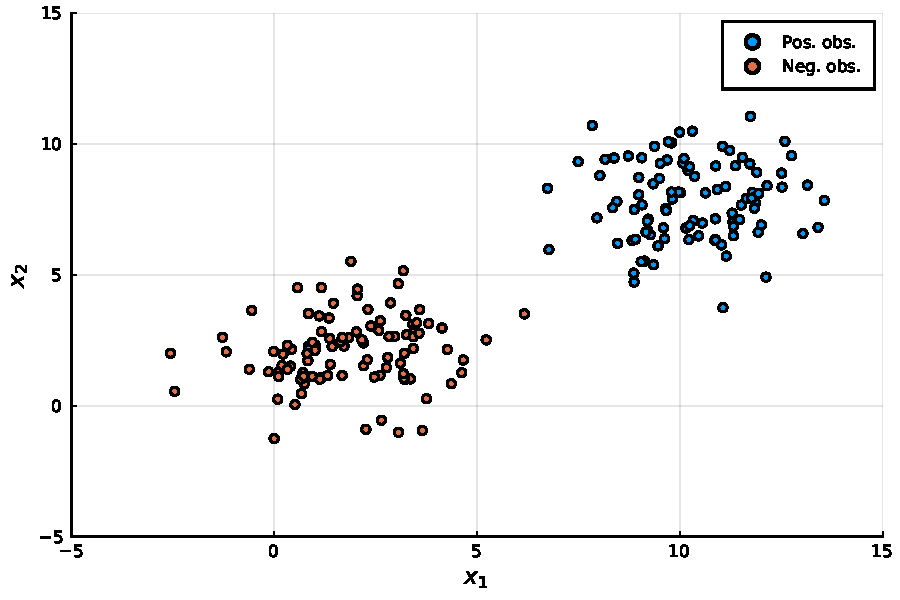
\includegraphics[width=0.8\textwidth]{part_2/chapter_1/figures/classes_no_classifier.pdf}
    \caption{Two hundred observations for $x_i$ classified to belong to $I^-$ (orange) or $I^+$ (blue).}        
    \label{fig:classified_observations}
\end{figure}

Our task is to obtain a function $f:\reals^n \mapsto \reals$ from a given family of functions that is capable to, given an observed set of features $\hat{x}$, classify whether it belongs to $I^-$ or $I^+$. In other words, we want to calibrate $f$ such that
%
\begin{align}
	f(x_i) < 0, \ \forall x_i \in I^-, \text{ and } f(x_i) > 0, \ \forall x_i \in I^+.  
\end{align}
%
This function would then act as a classifier that could be employed to any new observation $\hat{x}$ made. If $f$ is presumed to be an affine function of the form $f(x) = a^\top x - b$, then we obtain a \emph{linear classifier}. 

Our objective is to obtain $a \in \reals^n$ and $b \in \reals$ such that misclassification error is minimised. Let us define the error measure as
%
\begin{align*}
& e^-(x_i \in I^-; a, b) := 
    \begin{cases} 0, \text{ if } a^\top x_i - b \leq 0, \\
        a^\top x_i - b, \text{ if } a^\top x_i - b > 0.
    \end{cases} \\
& e^+(x_i \in I^+; a, b) := 
    \begin{cases} 0, \text{ if } a^\top x_i - b \geq 0, \\
        b -  a^\top x_i, \text{ if } a^\top x_i - b < 0.
    \end{cases}                   
\end{align*}
%
Using this error measure, we can define constraints that capture deviation on each measure by means of nonnegative slack variables. Let $u_i \geq 0$ for $i = 1, \dots, N$ and $v_i \geq 0$ for $i = 1,\dots, M$ be slack variables that measure the \emph{misclassification error} for $x_i \in I^-$ and $x_i \in I^+$, respectively.

The optimisation problem that finds optimal parameters $a$ and $b$ can be stated as
%
\begin{align}
	\mini \ & \sum_{i=1}^M u_i + \sum_{i=1}^N v_i \label{ex4:obj}\\
	\st & a^\top x_i - b - u_i \leq 0, i = 1, \dots, M \label{ex4:const1} \\
    & a^\top x_i - b + v_i \geq 0, i = 1,\dots,N \label{ex4:const2} \\
    & ||a||_2 = 1 \label{ex4:const3} \\
    & u_i \geq 0, i = 1, \dots, N \\
    & v_i \geq 0, i = 1, \dots, M \\
    & a \in \reals^n, b \in \reals. \label{ex4:end}   
\end{align} 
%
The objective function \eqref{ex4:obj} accumulates the total misclassification error. Constraint \eqref{ex4:const1} allows for capturing the misclassification error for each $x_i \in I^-$. Notice that $u_i = \max\braces{0, a^\top x_i -b} = e^-(x_i \in I^-; a, b)$. Likewise, constraint \eqref{ex4:const2} guarantees that $v_i = e^+(x_i \in I^+; a, b)$.
To avoid trivial solutions in which $(a,b) = (0, 0)$, the normalisation constraint $|| a ||_2 = 1$ is imposed in constraint \eqref{ex4:const3}, which turns the model nonlinear.

Solving the model \eqref{ex4:obj}--\eqref{ex4:end} provides optimal $(a,b)$ which translates into the classifier represented as the green line in Figure \ref{fig:observations_with_classifier}.

\begin{figure}[h]
    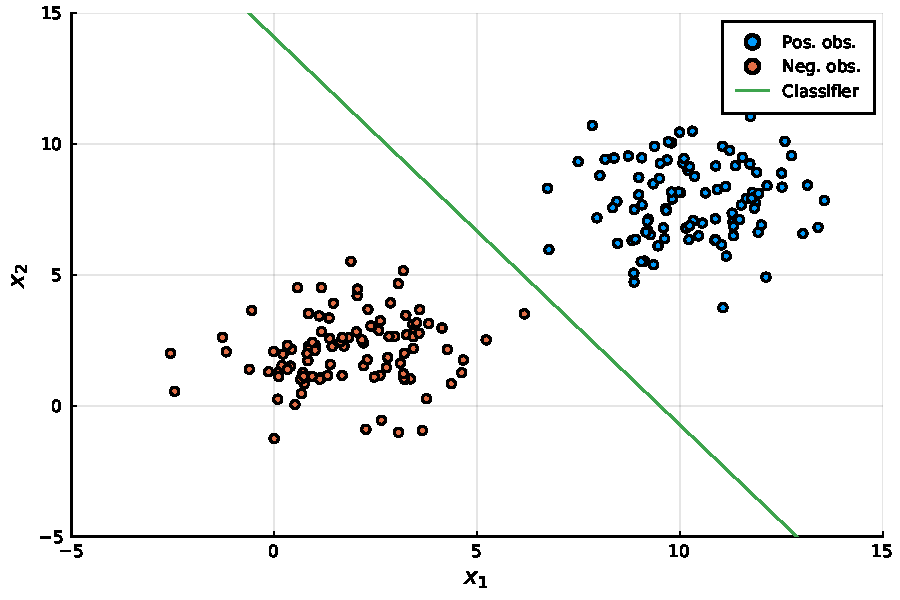
\includegraphics[width=0.8\textwidth]{part_2/chapter_1/figures/classes_with_classifier.pdf}
    \caption{Two hundred observations for $x_i$ classified to belong to $I^-$ (orange) or $I^+$ (blue) with a classifier (green).}        
    \label{fig:observations_with_classifier}
\end{figure}
 
A variant referred to as \emph{robust classifier} penalises not only the the misclassification error, but also the observations within a given slab $S = \braces{x \in \reals^n \mid -1 \leq a^\top x - b \leq 1}$. Notice that, being the two lines defined by $f^-(x) : a^\top x - b = -1$ and $f^+(x) : a^\top x - b = +1$, the distance between the two hyperplanes is given by $\frac{2}{||a||_2}$. 

Accordingly, we redefine our error measures as follows. 
%
\begin{align*}
	& e^-(x_i \in I^-; a, b) := 
	    \begin{cases} 0, \text{ if } a^\top x_i - b \leq -1, \\
	        |a^\top x_i - b|, \text{ if } a^\top x_i - b > -1.
	    \end{cases} \\
	& e^+(x_i \in I^+; a, b) := 
	    \begin{cases} 0, \text{ if } a^\top x_i - b \geq 1, \\
	        |b -  a^\top x_i|, \text{ if } a^\top x_i - b < 1.
	    \end{cases}                   
\end{align*}
%
By doing so, a penalty is applied not only to those points that were misclassified but also to those points correctly classified that happen to be inside the slab $S$. To define an optimal robust classifier, one must trade off the size of the slab, which is inversely proportional to $||a||$, and the total of observations that fall in the slab $S$. The formulation for the robust classifier then becomes
%
\begin{align}
	\mini \ & \sum_{i=1}^M u_i + \sum_{i=1}^N v_i + \gamma||a||_2^2 \label{ex5:obj}\\
	\st & a^\top x_i - b - u_i \leq -1, \ i = 1,\dots,M \label{ex5:const1} \\
	    & a^\top x_i - b + v_i \geq 1, \ i = 1,\dots,N \label{ex5:const2} \\
	    & u_i \geq 0, i = 1, \dots, N \\
	    & v_i \geq 0, i = 1, \dots, M \\
	    & a \in \reals^n, b \in \reals.
\end{align} 
%  
In objective function \eqref{ex5:obj}, the errors accumulated in variables $u_i$, $i=1,\dots,N$ and $v_i$, $i = 1,\dots,M$ and the squared norm $||a||_2^2$ are considered simultaneously. The term $\gamma$ is a scalar used to impose an emphasis on minimising the norm $||a||_2$ and incentivising a larger slab $S$ (recall that the slab is large for smaller $||a||_2$). The squared norm  $||a||_2^2$ is considered instead as a means to recover differentiability, as the norm  $||a||_2$ is not differentiable. Later on, we will see how beneficial it is for optimisation methods to be able to assume differentiability. Moreover, note how in constraints \eqref{ex5:const1} and \eqref{ex5:const2} $u$ and $v$ also accumulate penalties for correctly classified $x_i$ that happen to be between the slab $S$, that is, that have term $a^\top x - b$ larger/ smaller than -1/ +1. Figure \ref{fig:observations_with_rob_classifier} shows a robust classifier an arbitrary value of $\gamma$.

\begin{figure}[H]
    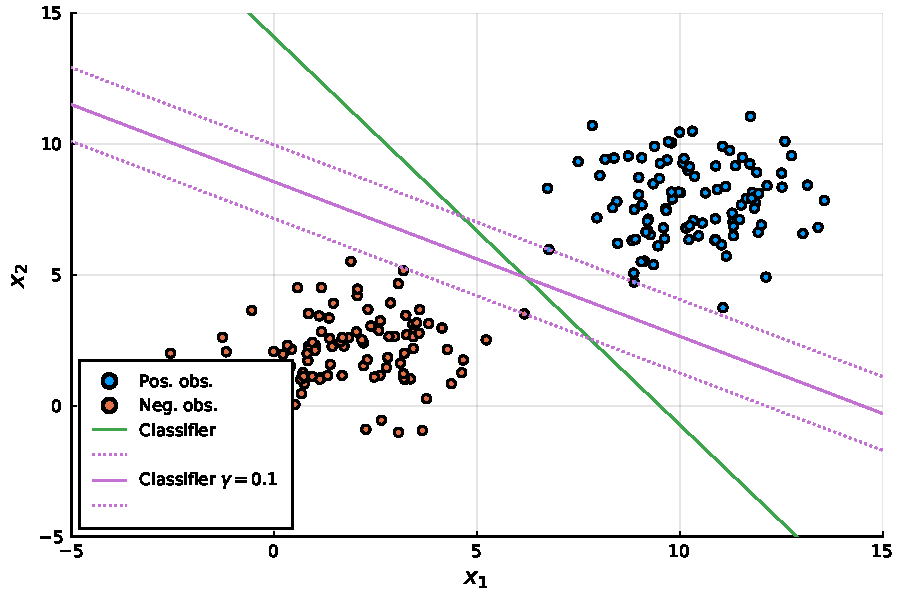
\includegraphics[width=0.8\textwidth]{part_2/chapter_1/figures/classes_with_robust_classifier.pdf}
    \caption{Two hundred observations for $x_i$ classified to belong to $I^-$ (orange) or $I^+$ (blue).}        
    \label{fig:observations_with_rob_classifier}
\end{figure}


{\bf Remark:} robust classifiers are known in the machine learning literature as \emph{support vector machines}, where the support vectors are the observations that support the slab. 

	
	\chapter{Decision Rules}
	

\section{Convexity and optimisation}

\emph{Convexity} is perhaps the most important property that the elements forming an optimisation problem can present. Paraphrasing Tyrrell Rockafellar:

\begin{quote}
... in fact, the great watershed in optimization isn't between linearity and nonlinearity, but convexity and nonconvexity.
\end{quote}

The importance of convexity will become clear later in the course. In a nutshell, the existence of convexity allows us to infer global properties of a solution (i.e., that holds for all of its domain) by considering exclusively local information (such as gradients, for example). This is critical in the context of optimisation, since most of the methods we know to perform well in practice are designed to find solutions that satisfy local optimality conditions. Once convexity is attested, one can then guarantee that these local solutions are in fact globally optimal without exhaustively exploring the solution space. 

For a problem of the form
% 
\begin{align*}
    (P) :~ \mini & f(x) \\
    \st & x \in X
\end{align*}
%
to be convex, we need to verify whether $f$ is a \emph{convex function} and $X$ is a \emph{convex set}. If both statements hold true, we can conclude that $P$ is a \emph{convex problem}. We start looking into how to identify convex sets, since we can use the convexity of sets to infer the convexity of functions.


\section{Identifying convexity of sets}
 
Before we formally define convex sets, let us first look at the idea of \emph{combinations}. For that, let $S \subseteq \reals^n$ be a set and $x_j \in S$ for $j=1,\dots,k$ be a collection of vectors (i.e., $n$-dimensional ``points'') belonging to $S$. Then, we have that:
%
\begin{itemize} 
	\item A \emph{linear combination} of $x_j$ for $j=1,\dots, k$ is the set 
%
	\begin{align}
		\braces{x \in \reals^n : \sum_{j=1}^k \lambda_jx_j, \ \lambda_j \in \reals \text{ for } j=1,\dots, k}.
	\end{align}
%
	\item An \emph{affine combination} is a linear combination, with the additional constraint that $\sum_{j=1}^k \lambda_j = 1$. That is,
%
	\begin{align}
		\braces{x \in \reals^n : \sum_{j=1}^k \lambda_jx_j, \ \sum_{j=1}^k \lambda_j = 1, \ \lambda_j \in \reals \text{ for } j=1, \dots, k}.
	\end{align}
%
	\item A \emph{conic combination} is a linear combination with the additional condition that $\lambda_j \geq 0$ for $j = 1,\dots,k$.
%
	\begin{align}
		\braces{x \in \reals^n : \sum_{j=1}^k \lambda_jx_j, \ \lambda_j \geq 0 \text{ for } j=1,\dots,k}.
	\end{align}
%
	\item And finally, a \emph{convex combination} is the intersection between an affine and a conic combinations, implying that $\lambda_j \in [0,1]$.  
%
	\begin{align}
		\braces{x \in \reals^n : \sum_{j=1}^k \lambda_jx_j, \ \sum_{j=1}^k \lambda_j = 1, \ \lambda_j \geq 0 \text{ for } j=1,\dots,k}.
	\end{align}
% 
\end{itemize}

We say that a set is convex if it contains all points formed by the convex combination of any pair of points in this set. This is equivalent to saying that the set contains the line segment between any two points belonging to the set. 

\begin{definition}[Convex sets] \label{def:convex_sets}
	A set $S \subseteq \reals^n$ is said to be convex if $\overline{x} = \sum_{j=1}^k \lambda_jx_j$ belongs to $S$, where $\sum_{j=1}^k \lambda_j = 1$, $\lambda_j \geq 0$ and $x_j \in S$ for $j=1,\dots, k$.
\end{definition}

Definition \ref{def:convex_sets} is useful as it allows for showing that some set operations preserve convexity. 

\subsection{Convexity-preserving set operations}

\begin{lemma}[Convexity-preserving operations] \label{lem:convex_operations}
	Let $S_1$ and $S_2$ be convex sets in $\reals^n$. Then, the sets resulting from the following operations are also convex.
	\begin{enumerate}
		\item {Intersection:} $S = S_1 \cap S_2$;
		\item {Minkowski addition:} $S = S_1 + S_2 = \braces{x_1 + x_2 : x_1 \in S_1, x_2 \in S_2}$;
		\item {Minkowski\hspace{-1pt} difference:}\hspace{-2pt} $S = S_1 - S_2 = \braces{x_1 - x_2 : x_1 \in S_1, x_2 \in S_2}$;
		\item {Affine transformation:} $S = \braces{Ax + b : x \in S_1}$.
	\end{enumerate}
\end{lemma}

Figures \ref{fig:mink_sum} and \ref{fig:intersection} illustrate the concept behind some of these set operations. Showing that the sets resulting from the operations in Lemma \ref{lem:convex_operations} are convex typically entails showing that convex combinations of elements in the resulting set $S$ also belong to $S_1$ and $S_2$.

\begin{figure}
	\centering
    	\begin{tikzpicture}
%    		\draw[help lines] (-6,-3) grid (6,3);
    		\node (picture) at (0,0) {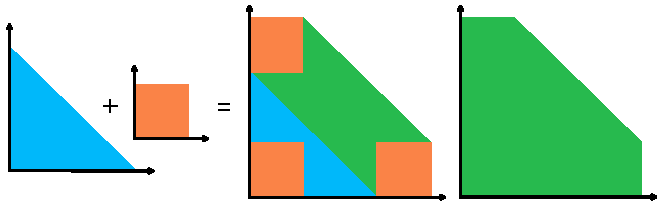
\includegraphics{part_2/chapter_2/figures/mink_sum}};
    		\node (A) at (-5, -0.5) {$S_1$};
    		\node (B) at (-2.9, -0.1) {$S_2$};
    		\node (C) at (-1, 1) {$S_2$};		
    		\node (D) at (-1, -1.1) {$S_2$};
    		\node (E) at (1.2, -1.1) {$S_2$};
    		\node (F) at (3, -0.5) {$S$};
    		\node (G) at (-1.1, -0.15) {$S_1$};
    	\end{tikzpicture}
		\caption{Minkowski sum of two convex sets.}\label{fig:mink_sum}
\end{figure}

%
\begin{figure}
	\centering
    \begin{tikzpicture}
%    		\draw[help lines] (-2,-2) grid (2,2);
    		\node (picture) at (0,0) {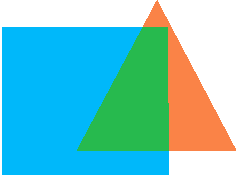
\includegraphics{part_2/chapter_2/figures/intersection.pdf}};
    		\node (A) at (-1, -0.15) {$S_1$};
    		\node (B) at (1.2, -0.5) {$S_2$};
    		\node (C) at (0.2, -0.8) {$S_1 \cap S_2$};
    \end{tikzpicture}
    
    \caption{Intersection of two convex sets.} \label{fig:intersection}
\end{figure}
%

\subsection{Examples of convex sets}

There are several familiar sets that are known to be convex. Having the knowledge that these sets are convex is useful as a building block for determining the convexity of more complicated sets.

Some important examples of convex sets include:
\begin{itemize}
	\item Them empty set $\emptyset$, any singleton $\{\overline{x}\}$ and the whole space $\reals^n$; 
	\item halfspaces: $S = \braces{x : p^\top x \leq \alpha} \subset \reals^n$;
	\item hyperplanes: $H = \braces{x : p^\top x = \alpha} \subset \reals^n$, where $p \neq 0^n$ is a normal vector and $\alpha\in \reals$ is a scalar. Notice that $H$ can be equivalently represented as $H = \braces{x \in \reals^n: p^\top(x - \overline{x}) = 0}$ for $\overline{x} \in H$;
	\item polyhedral sets: $P = \braces{x : Ax \leq b} \subset \reals^n$, where $A\in \reals^{m\times n}$ and $b \in \reals^n$;
	\item norm-induced sets (balls): $B = \braces{x : ||x - \overline{x}|| \leq \alpha} \subseteq \reals^n$, where $|| \cdot ||$ is any norm and $\alpha$ a scalar;
	\item norm cones: $C =\braces{(x,\alpha) \in \reals^{n+1}: ||x|| \leq \alpha} $;
\end{itemize} 

For example, let us consider the polyhedral set $P = \braces{x \in \reals^n : Ax \leq b} \subset \reals^n$ with $A$ being a $m \times n$ matrix. Notice that $S$ is the intersection of a collection of half-spaces $H_i = \braces{x \in \reals^n : a_i^\top x \leq b_i}$, where $a_i$ are vectors from the rows of the matrix $A$ and $b_i$ are the components of the column vector $b$. We know that $H_i$ are convex sets, thus $P = \cap_{i=1}^m H_i$ is also convex, as the intersection of sets is a convexity-preserving set operation.


\subsubsection{Hyperplanes and halfspaces}

Hyperplanes and halfspaces will play a central role in the developments we will see in our course. Therefore, let us take a moment and discuss some important aspects related these convex sets. First, notice that, geometrically, a hyperplane $H \subset \reals^n$ can be interpreted as the set of points with a \emph{constant} inner product to a given vector $p \in \reals^n$, while $\overline{x}$ determines the offset of the hyperplane from the origin. That is,
	\begin{equation*}
		H = \braces{x : p^\top(x - \overline{x}) = 0} \equiv \overline{x} + p^{\perp},
	\end{equation*}
	where $p^\perp$ is the orthogonal complement of $p$, i.e., the set of vectors orthogonal to $p$, which is given by $\braces{x \in \reals^n : p^\top x = 0}$.
	
	\begin{figure}[H]
	    \begin{tikzpicture}
%    		\draw[help lines] (-2,-2) grid (2,2);
    		\node (picture) at (0,0) {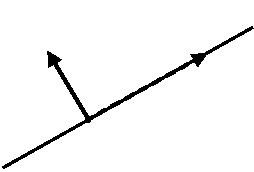
\includegraphics{part_2/chapter_2/figures/hyperplane.pdf}};
    		\node (p) at (-1.3, 0.8) {$p$};
    		\node (xbar) at (-0.6, -0.8) {$\overline{x}$};
    		\node (H) at (2, 0.5) {$H$};
		\end{tikzpicture}
		\caption{A hyperplane $H = \braces{x \in \reals^n: p^\top(x - \overline{x}) = 0}$ with normal vector $p$ displaced to $\overline{x}$.}
	\end{figure}
	
	Analogously, a halfspaces can be represented as $S = \braces{x \in \reals^n : p^\top(x - \overline{x}) \le 0}$ where $p^\top \overline{x} = \alpha$ is the hyperplane that forms the boundary of the halfspace. This definition suggests a simple geometrical interpretation: the halfspace $S$ consists of $\overline{x}$ plus any vector with an obtuse or right angle (i.e., greater of equal to 90$^\circ$) with the outward normal vector $p$.
 
 	\begin{figure}[H]
	    \begin{tikzpicture}
%    		\draw[help lines] (-2,-2) grid (2,2);
    		\node (picture) at (0,0) {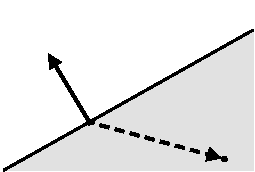
\includegraphics{part_2/chapter_2/figures/halfspace.pdf}};
    		\node (p) at (-1.3, 0.75) {$p$};
    		\node (xbar) at (-0.6, -0.9) {$\overline{x}$};
    		\node (x) at (1.9, -1.3) {$x$};
    		\node (H) at (1.7, 0.3) {$S$};
		\end{tikzpicture}
		\caption{A halfspace $S = \braces{x \in \reals^n : p^\top(x - \overline{x}) \le 0}$ defined by the same hyperplane $H$. Notice how the vectors $p$ (or $p - \overline{x}$, which is fundamentally the same vector but translated to $\overline{x}$) and $x - \overline{x}$ form angles greater or equal than $90^\circ$.}
	\end{figure}
	
	\begin{figure}[H]
    \begin{tikzpicture}
%    		\draw[help lines] (-2,-2) grid (2,2);
    		\node (picture) at (0,0) {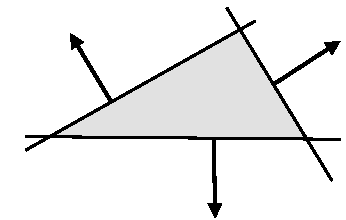
\includegraphics{part_2/chapter_2/figures/polyhedral_set.pdf}};
    		\node (P) at (0.75, 0.25) {$P$};
    		\node (a1) at (-1.6, 1.4) {$a_1$};
    		\node (a2) at (1, -1.8) {$a_2$};    		
    		\node (a2) at (2.8, 1.3) {$a_3$};
    \end{tikzpicture}
    \caption{A polyhedron $P$ formed by the intersection of three halfspace. Each hyperplane $H_i = \braces{x \in \reals^n : a_i^\top x \leq b_i}$, for $i = 1,2,3$, has a normal vector $a_i$, and has an offset from the origin $b_i$ (which cannot be seen once project on a 2-dimensional plane as in the picture).} \label{fig:polyhedral_set}
\end{figure}

\subsubsection{Norm balls and norm cones}

An Euclidean ball (or simply ball) of radius $\epsilon$ in $\reals^n$ has the form
%
\begin{equation*}
	B(\overline{x}, r) = \braces{x \in \reals^n : || x - \overline{x}||_2 \le \epsilon} \equiv \braces{x \in \reals^n : (x - \overline{x})^\top (x - \overline{x}) \le \epsilon^2}
\end{equation*}
%
As one might suspect, balls are convex, which can be proved by noting that
%
\begin{align*}
	||\lambda x_1 + (1 - \lambda) x_2 - \overline{x}||_2  & = ||\lambda (x_1 - \overline{x}) + (1 - \lambda) (x_2 - \overline{x})||_2 \\
	& \le \lambda ||x_1 - \overline{x}||_2 + + (1 - \lambda) ||x_2 - \overline{x}||_2 \le \epsilon.
\end{align*}
%
Notice that between the first and the second line, we use the triangle inequality, which states that $||x + y|| \le ||x|| + ||y||$ for any two vectors $x$ and $y$ and any norm (including the Euclidean norm). 

Euclidean balls are a special case of norm balls, which are defined as $B(\overline{x}, r) = \braces{x \in \reals^n : || x - \overline{x}|| \le \epsilon}$ where $||\ \cdot \ ||$ is any norm on $\reals^n$. 

A related set is the norm cone, defined as $C(x, \alpha) = \braces{(x,\alpha) \in \reals^{n+1} : ||x|| \le \alpha}$, where $\alpha$ is a scalar. For example, the second-order cone (also known as the ice cream cone or Lorentz cone) is the norm cone for the Euclidean norm.

\begin{remark} 
	Norm induced sets (balls or cones) are convex for any norm $||x||_p = \left(\sum_{i=1}^n x_i^p\right)^{\frac{1}{p}}$ for $x \in \reals^n$ and $p \geq 1$.
\end{remark}


\section{Convex hulls} 

A \emph{convex hull} of a set $S$, denoted $\conv(S)$ is the set formed by all convex combinations of all points in $S$. As the name suggests, $\conv(S)$ is a convex set, regardless of $S$ being or not convex. 

Another interpretation for $\conv(S)$ is to think of it as the tightest enveloping (convex) set that contains $S$. Notice that, if $S$ is convex, then $S = \conv(S)$.  Formally, convex hulls are defined as follows.

\begin{definition}[Convex hull of a set]\label{def: convex_hull}
	Let $S \subseteq \reals^n$ be an arbitrary set. The convex hull of $S$, denoted by $\conv(S)$, is the collection of all convex combinations of $S$. That is, for $x_j \in S$, with $j = 1,\dots, k$, $x \in \conv(S)$ if and only if 
	%
	\begin{equation*}
		x = \sum_{j=1}^k \lambda_jx_j : \sum_{j=1}^k \lambda_j = 1, \ \lambda_j \geq 0, \text{ for } j = 1,\dots,k.
	\end{equation*}                       
	%
\end{definition}
%

From Definition \ref{def: convex_hull}, one can show that the convex hull $\conv(S)$ can also be defined as the intersection of all convex sets containing $S$. Perhaps the easiest way to visualise this is to think of the infinitely many half-space containing $S$ and their intersection, which can only be $S$. Figure \ref{fig:convex_hull} illustrates the convex hull $\conv(S)$ of an nonconvex set $S$.
%
\begin{figure}[H]
%
\includegraphics[width=0.3\textwidth]{Figures/convex_hull.pdf}
	\begin{tikzpicture}
%    		\draw[help lines] (-3,-2) grid (3,2);
    		\node (picture) at (0,0) {
\includegraphics{part_2/chapter_2/figures/convex_hull.pdf}};
    		\node (A) at (-1.5, 0) {$S$};
    		\node (B) at (0.3, 0.5) {$\conv(S)$};
    \end{tikzpicture}
\caption{Example of an arbitrary set $S$ (in solid blue) and its convex hull $\conv(S)$ (combined blue and grey areas).} \label{fig:convex_hull}
\end{figure}
%
The notion of convex hulls is a powerful tool in optimisation. One important application is using $\conv(S)$ to obtain approximations for a nonconvex $S$ that can be exploited to solve an optimisation problem with constraint set defined by $S$. This is the underpinning technique in many important optimisation methods for such as branch-and-bound-based methods for nonconvex problems and decomposition methods (i.e., methods that solve large problems by breaking it into smaller parts that are presumably easier to solve).  

In specific, let us consider the convex hull of a finite collection of discrete points. Some of these sets are so important in optimisation that they have their own names. 
%
\begin{definition}
Let $S = \braces{x_1, \dots, x_{n+1}} \subset \reals^n$. Then $\conv(S)$ is called a \emph{polytope}. If $x_1,\dots,x_{n+1}$ are affinely independent (i.e., $x_2 - x_1, \dots ,x_{n+1} - x_1$ are linearly independent) then $\conv(S)$ is called a \emph{simplex} with vertices $x_1,\dots,x_{n+1}$.
\end{definition}
%


%\subsection{The Carath\'eodory theorem*}
%
%
%The \emph{Carath\'eodory theorem} is an important result associated with simplexes. It states that if $x \in \conv(S) \subset \reals^n$, then there exists a simplex composed by $x_j \in S$ for $j = 1, \dots, n+1$ that contains $x$. Formally, the theorem is posed as follows.
%%
%\begin{theorem}[Carath\'eodory theorem]
%Let $S \subseteq \reals^n$. If $x \in \conv(S)$, then $x \in \conv(x_1, \dots, x_{n+1})$ for some $x_j \in S$ where $j = 1,\dots, n+1$.        
%\end{theorem}   
%
%%% Consider including a proof for the Caratheodory theorem, for the sake of completeness.
%
%
%More specifically, any point $x \in \conv(S)$ can be expressed as
%%
%\begin{equation*}
%	x = \sum_{j=1}^{n+1} \lambda_jx_j : \sum_{j=1}^{n+1} \lambda_j = 1, \ \lambda_j \geq 0, \text{ for } j = 1,\dots,{n+1},
%\end{equation*}
%%
%for a given collection of points $x_j$, with $j = 1, \dots, n+1$ forming a simplex. Figure \ref{fig:caratheodory} illustrates this result.
%%
%\begin{figure}[h]
%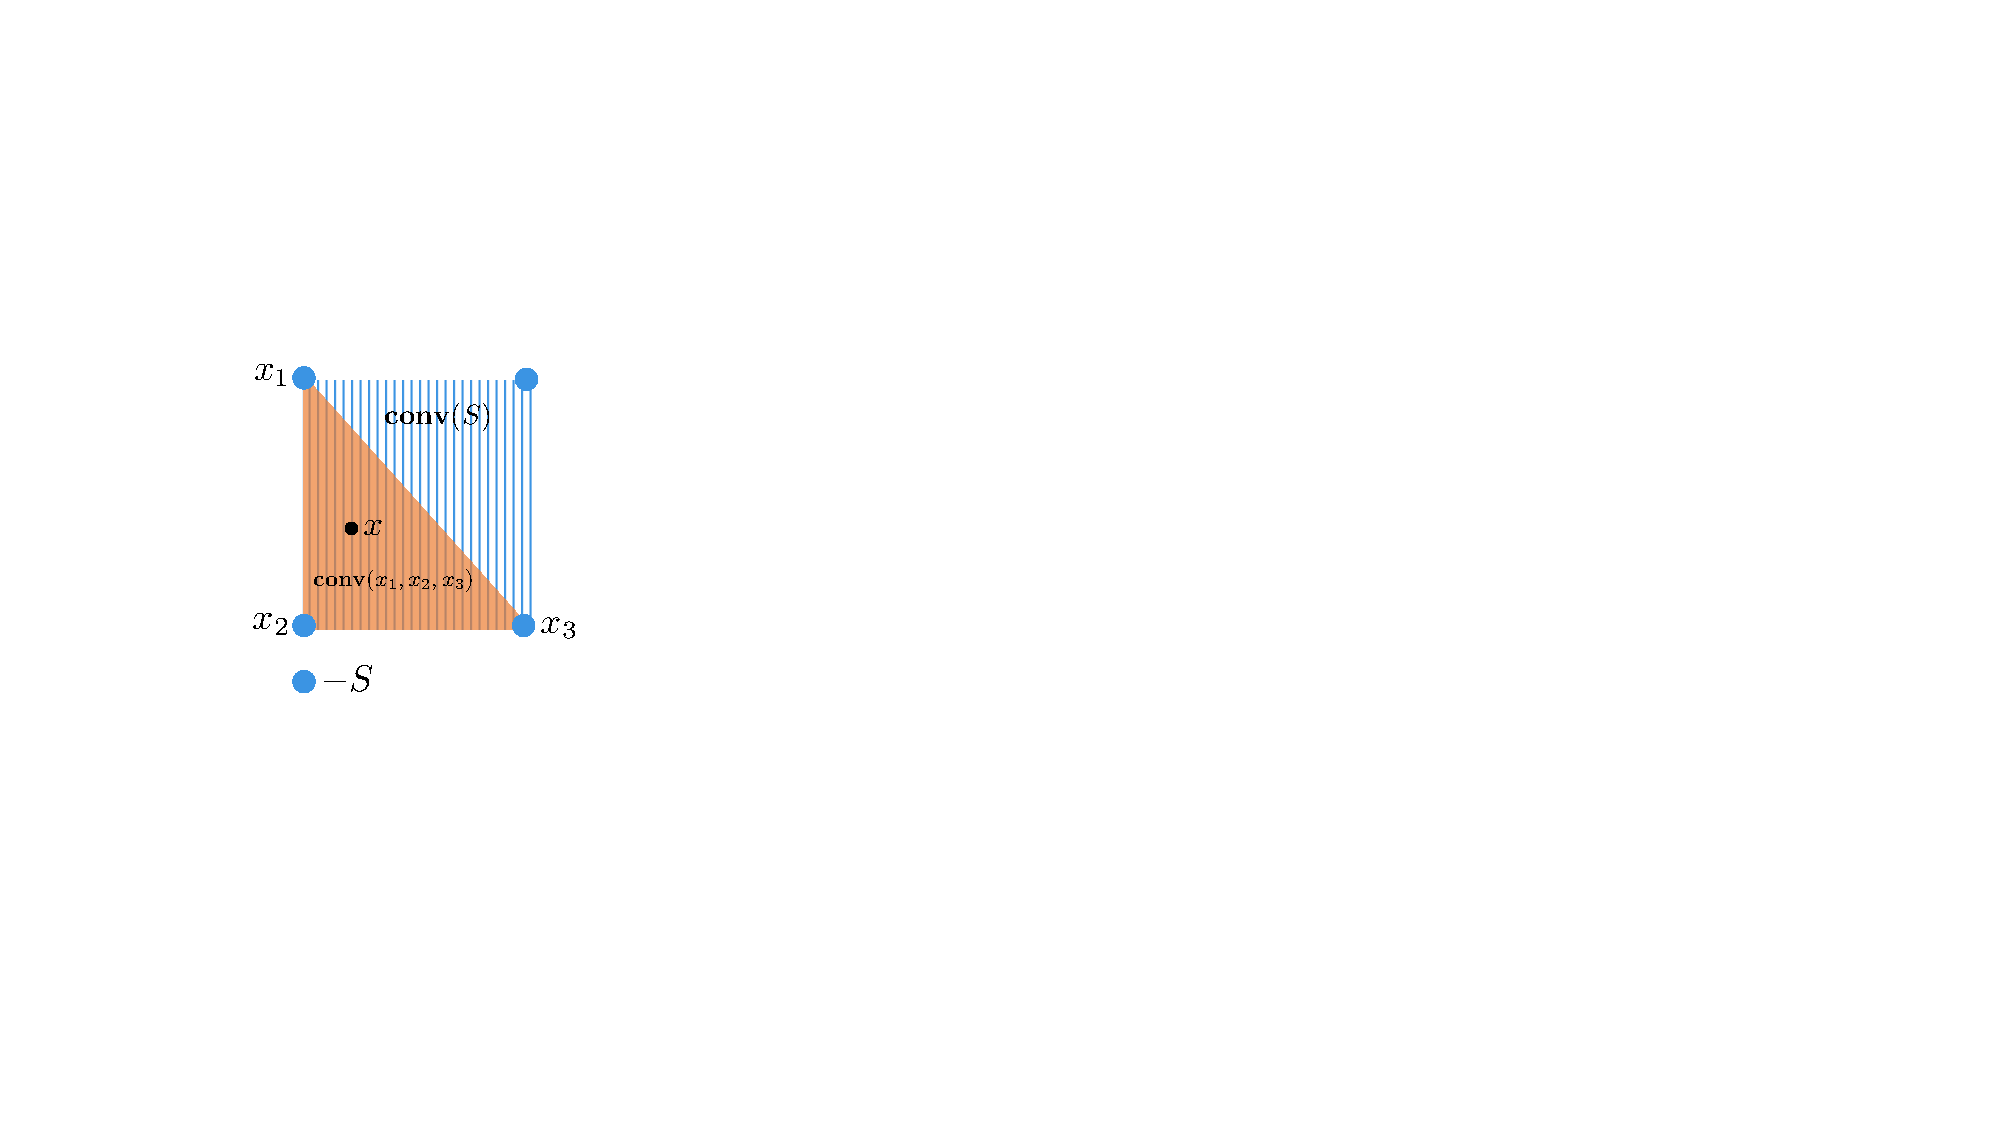
\includegraphics[width=0.3\textwidth]{Figures/caratheodory.pdf}
%\caption{Example of an arbitrary set $S$ (blue dots) and its convex hull $\conv(S)$ (light blue). Notice that $x$ can be represented as the convex combination of $x_j$ for $j=1,2,3$ for $n=2$.} \label{fig:caratheodory}
%\end{figure} 


\section{Closure and interior of sets}

Many of the set-related results we will see in this course depends on the characteristics of the set itself. Often, assuming properties such as closedness or compactness considerably ease technical derivations. 


\subsection{Closure, interior and boundary of a set}


Let us define some properties that will be useful in this course. For that, we will use an $\epsilon$-neighbourhood of $x \in \reals^n$ (which is a norm ball of radius $\epsilon$ centred in $x$) defined as
%
\begin{align*}
    N_\epsilon(x) = \braces{y : ||y - x|| < \epsilon}.
\end{align*}
%
Let $S \subseteq \reals^n$ be an arbitrary set. We can use $N_\epsilon$ to define the following elements related to $S$.  
\begin{enumerate}
\item \emph{Closure of $S$}: the set defined by the closure of $S$, denoted $\clo(S)$, is defined as 
%
\begin{align*}
\clo(S) = \braces{x \in \reals^n : S \cap N_\epsilon(x) \neq \emptyset \text{ for every } \epsilon > 0}. 
\end{align*}
%
Notice that the closure might contain points that do not belong to $S$. We say that a set is \emph{closed} if $S = \clo(S)$, that is, the set itself is its own closure. 
%
\item \emph{Interior of $S$}: the interior of $S$, denoted $\intr(S)$, is the set
\begin{align*}
\intr{S} = \braces{x \in S : N_\epsilon(x) \subset S \text{ for some } \epsilon > 0}.
\end{align*}
%
If $S$ is the same as its own interior, then we say that $S$ is \emph{open}. Some authors say that $S$ is solid if it has a nonempty interior (that is, $\intr(S) \neq \emptyset$. Notice that the interior of $S$ is a subset of $S$, that is $\intr(S) \subseteq S$.
%
\item \emph{Boundary of $S$}: the boundary of $S$, denoted $\bou(S)$ is the collection of points defined by
%
\begin{align*}
\bou(S) = \braces{x \in \reals^n : N_\epsilon(x) \text{ contains some } x_i \in S \text{ and some } x_j \notin S \text{ for every } \epsilon > 0}.
\end{align*}
%
We say that $S$ is bounded if exists $N_\epsilon(x)$, $x \in \reals^n$, for some $\epsilon > 0$ such that $S \subset N_\epsilon(x)$. 
\end{enumerate}

We say that a set is \emph{compact} if it is both \emph{closed} and \emph{bounded}. Compact sets appear very frequently in real-world applications of optimisation, since typically one can assume the existence of bounds for decision variables (such as nonnegativity or maximum physical bounds or, at an extreme case, smallest/ largest computational constants). Another frequent example of bounded set is the convex hull of a collection of discrete points, which is called by some authors \emph{polytopes} (effectively bounded polyhedral sets).  

Let us consider the following example. Let $S = \braces{(x_1,x_2) \in \reals^n : x_1^2 + x_2^2 \leq 1}$. Then, we have that:
\begin{enumerate}
	\item $\clo(S) = \braces{(x_1,x_2) \in \reals^n : x_1^2 + x_2^2 \leq 1}$. Since $S = \clo(S)$, $S$ is closed.
	\item $\intr(S) = \braces{(x_1,x_2) \in \reals^n : x_1^2 + x_2^2 < 1}$. 
	\item $\bou(S) = \braces{(x_1,x_2) \in \reals^n : x_1^2 + x_2^2 = 1}$. Notice that it makes $S$ bounded.
	\item $S$ is compact, since it is closed and bounded. 
\end{enumerate}

Notice that, if $S$ is closed, then $\bou(S) \subset S$. That is, its boundary is part of the set itself. Moreover, it can be shown that $\clo(S) = \bou(S) \cup S$ is the smallest closed set containing $S$. 

In case $S$ is convex, one can infer the convexity of the interior $\intr(S)$ and its closure $\clo(S)$. The following theorem summarises this result.
%
\begin{theorem}\label{thm:top_convex_comb}
Let $S \subseteq \reals^n$ be a convex set with $\intr(S) \neq \emptyset$. Let $x_1 \in \clo(S)$ and $x_2 \in \intr(S)$. Then $x = \lambda x_1 + (1 - \lambda) x_2 \in \intr(S)$ for all $\lambda \in (0,1)$.
\end{theorem}
%

% Consider including the proof for this theorem (on page 46)

Theorem \ref{thm:top_convex_comb} is useful for inferring the convexity of the elements related to $S$. We summarise the key results in the following corollary.
%
\begin{corollary} Let $S$ be a convex set with $\intr(S) \neq \emptyset$. Then
	\begin{enumerate}
		\item $\intr(S)$ is convex;
		\item $\clo(S)$ is convex;
		\item $\clo(\intr(S)) = \clo(S)$;
		\item $\intr(\clo(S)) = \intr(S)$.
	\end{enumerate}
\end{corollary}
%

% Consider including the proof for this corollary (on page 46)


\subsection{The Weierstrass theorem}


The Weierstrass theorem is a result that guarantees the existence of optimal solutions for optimisation problems. To make it more precise, let
%
\begin{align*}
	(P) :~ z = \mini\braces{f(x) : x \in S}  
\end{align*}
%
be our optimisation problem. If an optimal solution $x^*$ exists, then $f(x^*) \leq f(x)$ for all $x \in S$ and $z = f(x^*) = \min \braces{f(x) : x \in S}$. 

Notice the difference between $\mini$ (an abbreviation for minimise) and the operator $\min$. The first is meant to represent the problem of minimising the function $f$ in the domain $S$, while $\min$ is shorthand for minimum, in this case $z$, assuming that it is attainable.

It might be that an optimal solution is not attainable, but a bound can be obtained for the optimal solution value. The greatest lower bound for $z$ is its \emph{infimum} (or \emph{supremum} for maximisation problems), denoted by $\inf$. That is, if $z = \inf\braces{f(x) : x \in S}$ , then $z \leq f(x)$ for all $x \in S$ and there is no $\overline{z} > z$ such that $\overline{z} \leq f(x)$ for all $x \in S$. We might sometimes use the notation 
%
\begin{align*}
(P) :~ z = \inf\braces{f(x) : x \in S}
\end{align*}
%
to represent optimisation problems for which one cannot be sure whether an optimal solution is attainable. The Weierstrass theorem describes the situations in which those minimums (or maximums) are guaranteed to be attained, which is the case whenever $S$ is compact.
%
\begin{theorem}[Weierstrass theorem]\label{thm:weierstrass}
Let $S \neq \emptyset$ be a compact set, and let $f:S \rightarrow \reals$ be continuous on $S$. Then there exists a solution $\overline{x} \in S$ to $\mini\braces{f(x) : x \in S}$. 
\end{theorem}
%
Figure \ref{fig:Weierstrass} illustrates three examples. In the first (on the left) the domain $[a,b]$ is compact, and thus the minimum of $f$ is attained at $b$. In the other two, $[a,b)$ is open and therefore, Weierstrass theorem does not hold. In the middle example, one can obtain $\inf f$, which is not the case for the last example on the right.
%
\begin{figure}[h]
%\includegraphics[width=0.8\textwidth]{Figures/Weierstrass.pdf}
	\begin{tikzpicture}
%    		\draw[help lines] (-6,-1) grid (6,1);
    		\node (picture) at (0,0) {\includegraphics{part_2/chapter_2/figures/Weierstrass.pdf}};
    		\node (fa1) at (-5.8, 0.75) {$f(a)$};
    		\node (fb1) at (-5.8, -0.8) {$f(b)$};
 	    		\node (fa2) at (-1.8, 0.75) {$f(a)$};
    		\node (fb2) at (-1.8, -0.8) {$\inf f$};
 	    		\node (fa3) at (2.2, 0.75) {$f(a)$};
 	    		\node (a1) at (-5, -1.55) {$a$};
    		\node (b1) at (-3, -1.55) {$b$};
    		\node (a2) at (-1, -1.55) {$a$};
    		\node (b2) at (1, -1.55) {$b$};
 	    		\node (a3) at (3, -1.55) {$a$};
    \end{tikzpicture}
	\caption{Examples of attainable minimum (left) and infimum (centre) and an example where neither are attainable (right).} \label{fig:Weierstrass}
\end{figure}


\section{Separation and support of sets}
 

The concepts of \emph{separation} and \emph{support} of sets are key for establishing optimality conditions later in this course. We are interested in mechanisms that allow one to infer whether there exists hyperplanes separating points from sets (or sets from sets). We will also be interested in means to, given a point $x \notin S$, find the closest to point not belonging to $S$.

\subsection{Hyperplanes and closest points}

We start with how to identify closest points to sets. 
%
\begin{theorem}[Closest-point theorem]\label{thm:closest_point}
Let $S \neq \emptyset$ be a closed convex set in $\reals^n$ and $y \notin S$. Then, there exists a unique point $\overline{x} \in S$ with minimum distance from $y$. In addition, $\overline{x}$ is the minimising point if and only if $$(y-\overline{x})^\top(x - \overline{x}) \leq 0, \text{ for all } x\in S$$
\end{theorem}
%
Simply put, if $S$ is a closed convex set, then $\overline{x} \in S$ will be the closest point to $y \notin S$ if the vector $y - \overline{x}$ is such that if it forms an angle that is greater or equal than 90$^\circ$ with all other vectors $x - \overline{x}$ for $x \in S$. Figure \ref{fig:closest_point} illustrates this logic. 

\begin{figure}[h]
	\begin{tikzpicture}
%    	\draw[help lines] (-3,-2) grid (3,2);
		\node (picture) at (0,0) {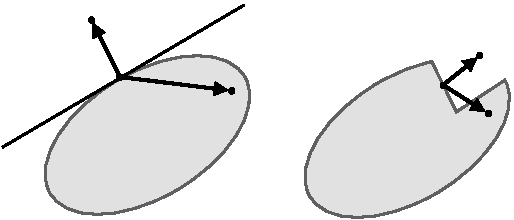
\includegraphics{part_2/chapter_2/figures/closest_point.pdf}};
		\node (y1) at (-2.8, 2) {$y$};
		\node (y2) at (4, 0.8) {$y$};
		\node (xbar1) at (-2.6, 0.4) {$\overline{x}$};
		\node (xbar2) at (2.9, 0.3) {$\overline{x}$};
		\node (x1) at (-0.4, -0.1) {$x$};    		
		\node (x2) at (3.9, -0.5) {$x$};
		\node (S) at (-2, -1) {$S$};
		\node (S) at (2, -1) {$S$};    		
    \end{tikzpicture}
	\caption{Closest-point theorem for a closed convex set (on the left). On the right, an illustration on how the absence of convexity invalidates the result.} \label{fig:closest_point}
\end{figure}

Notice that $S$ lies in the half-space $(y-\overline{x})^\top(x - \overline{x}) \leq 0$ defined by the hyperplane $p^\top(x - \overline{x}) =0$ with normal vector $p = (y - \overline{x})$. We will next revise the concepts of half-spaces and hyperplanes, since they will play a central role in the derivations in this course.  

\subsection{Halfspaces and separation}

We can use halfspaces to build the concept of separation. Let us start recalling that a hyperplane $H = \braces{x : p^\top x = \alpha}$ with normal vector $p \in \reals^n$ and $\alpha \in \reals$ defines two half-spaces $H^+ = \braces{x : p^\top x \geq \alpha}$ and $H^- = \braces{x : p^\top x \leq \alpha}$. Figure \ref{fig:hyperplane} illustrates the concept. Notice how the vector $p$ lies in the half-space $H^+$.
%
\begin{figure}
%	\includegraphics[scale=0.6]{Figures/hyperplanes.pdf}
	\begin{tikzpicture}
%    	\draw[help lines] (-2,-2) grid (2,2);
		\node (picture) at (0,0) {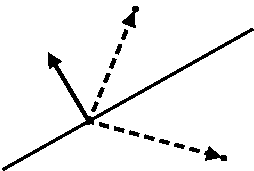
\includegraphics{part_2/chapter_2/figures/halfspaces.pdf}};
		\node (p) at (-1.4, 0.8) {$p$};
		\node (xbar) at (-0.7, -0.9) {$\overline{x}$};
		\node (H+) at (2, 1.2) {$H^{+}$};
		\node (H-) at (2, 0.5) {$H^{-}$};
	\end{tikzpicture}	
	\caption{Normal vectors, hyperplane and halfspaces} \label{fig:hyperplane}
\end{figure}
 
Any hyperplane $H$ can be defined in reference to a point $\overline{x} \in H$ by noticing that 
%
\begin{align*}
	p^\top(x - \overline{x}) = p^\top x - p^\top \overline{x} = \alpha - \alpha = 0.  
\end{align*}
%
From that, the half-spaces defined by $H$ can be equivalently stated as $H^+ = \braces{x : p^\top (x - \overline{x}) \geq 0}$ and $H^- = \braces{x : p^\top (x - \overline{x}) \leq 0}$.

We can now define the separation of convex sets. 
%
\begin{definition} \label{def:separation}
	Let $S_1$ and $S_2$ be nonempty sets in $\reals^n$. The hyperplane $H = \braces{x: p^\top x = \alpha}$ is said to \emph{separate} $S_1$ and $S_2$ if $ p^\top x \geq \alpha$ for each $x \in S_1$ and $p^\top x \leq \alpha$ for each $x \in S_2$. In addition, the following apply: 
	\begin{enumerate}
		\item {\bf Proper separation:} $S_1 \cup S_2 \not\subset H$;
		\item {\bf Strict separation:} $ p^\top x < \alpha$ for each $x \in S_1$ and $p^\top x > \alpha$ for each $x \in S_2$;
		\item {\bf Strong separation:} $ p^\top x \geq \alpha + \epsilon$ for some $\epsilon >0$ and $x \in S_1$, and $p^\top x \leq \alpha$ for each $x \in S_2$.
	\end{enumerate}
\end{definition}
%
Figure \ref{fig:separation} illustrates the three types of separation in Definition \ref{def:separation}. On the left, proper separation is illustrated, which is obtained by any hyperplane that does not contain both $S_1$ and $S_2$, but that might contain points from either or both. In the middle, sets $S_1$ and $S_2$ belong to two distinct half-spaces in a strict sense. On the right, strict separation holds with an additional margin $\epsilon > 0$, which is defined as strong separation. 
%
\begin{figure}[H]
%	\includegraphics[scale=0.8]{Figures/separations.pdf}
	\begin{tikzpicture}
%    	\draw[help lines] (-4,-2) grid (4,2);
		\node (picture) at (0,0) {\includegraphics{part_2/chapter_2/figures/separations.pdf}};
		\node (S11) at (-3.6, 0.5) {$S_1$};
		\node (S21) at (-3.15, -0.45) {$S_2$};
		\node (S12) at (-0.2, 0.5) {$S_1$};
		\node (S22) at (0.25, -0.45) {$S_2$};
		\node (S13) at (3, 0.5) {$S_1$};
		\node (S23) at (3.65, -0.45) {$S_2$};
		\node (H1) at (-2, 1.1) {$H$};		
		\node (H2) at (1.3, 1.1) {$H$};
		\node (H3) at (4.7, 1.1) {$H$};
	\end{tikzpicture}	
	\caption{Three types of separation between $S_1$ and $S_2$.} \label{fig:separation}
\end{figure}
%
A powerful yet simple result that we will use later is that, for a closed convex set $S$, there always exists a hyperplane separating $S$ and a point $y$ that does not belong to $S$.
%4
\begin{theorem}[Separation theorem]\label{p2c2:thm:separation}
Let $S \neq \emptyset$ be a closed convex set in $\reals^n$ and $y \notin S$. Then, there exists a nonzero vector $p \in \reals^n$ and $\alpha \in \reals$ such that $p^\top x \leq \alpha$ for each $x \in S$ and $p^\top y > \alpha$.
\end{theorem}
%
\begin{proof}
	Theorem \ref{thm:closest_point} guarantees the existence of a unique minimising $\overline{x} \in S$ such that $(y-\overline{x})^\top(x - \overline{x}) \leq 0$ for each $x \in S$. Let $p = (y - \overline{x}) \neq 0$ and $\alpha = \overline{x}^\top(y - \overline{x}) = p^\top\overline{x}$. Then we get $p^\top x \leq \alpha$ for each $x \in S$, while $p^\top y - \alpha = (y - \overline{x})^\top(y - \overline{x}) = ||y - \overline{x}||^2 > 0$.
\end{proof}

This is the first proof we look at in these notes, and the reason for that is its importance in many of the results we will discuss further. The proof first looks at the problem of finding a minimum distance point as an optimisation problem and uses the Weierstrass theorem (our Theorem \ref{thm:closest_point} is a consequence of the Weierstrass theorem stated in Theorem \ref{thm:weierstrass}) to guarantee that such a $\overline{x}$ exists. Being a minimum distance point, we know from Theorem \ref{thm:closest_point} that $(y-\overline{x})^\top(x - \overline{x}) \leq 0$ holds. Now by defining $p$ and $\alpha$ as in the proof, one might notice that
%
\begin{align*}
	& (y-\overline{x})^\top(x - \overline{x}) \leq 0 \ \Leftrightarrow \ 
	(y-\overline{x})^\top x \leq (y - \overline{x})^\top\overline{x} \ \Leftrightarrow \ 
	p^\top x \leq p^\top\overline{x} = \alpha. 
\end{align*}
%
The inequality $p^\top y > \alpha$ is demonstrated to hold in the final part by noticing that 
%
\begin{align*}
	p^\top y - \alpha &= 
	(y - \overline{x})^\top y - \overline{x}^\top(y - \overline{x}) \\ &= 
	y^\top(y - \overline{x}) - \overline{x}^\top(y - \overline{x}) \\ & = (y - \overline{x})^\top (y - \overline{x}) = || y - \overline{x} ||^2 > 0.
\end{align*}

Theorem \ref{thm:separation} has interesting consequences. For example, one can apply it to every point in the boundary $\bou(S)$ to show that $S$ is formed by the intersection of all half-spaces containing $S$. 

Another interesting result is the existence of strong separation. If $y \notin \clo(\conv(S))$, then one can show that strong separation between $y$ and $S$ exists since there will surely be a distance $\epsilon>0$ between $y$ and $S$. 


\subsection{Farkas' theorem}

Farkas' theorem plays a central role in deriving optimality conditions. It can assume several alternative forms, which are typically referred to as Farkas' lemmas. In essence, the Farkas' theorem is used to demonstrate that a given system of linear equations has a solution if and only if a related system can be shown to have no solutions and vice-versa. 

\begin{theorem}
	Let $A$ be an $m \times n$ matrix and $c$ be an $n$-vector. Then exactly one of the following two systems has a solution:
	%
	\begin{align*}
		(1) :~ &Ax \leq 0, \ c^\top x > 0, \ x \in \reals^n\\
		(2) :~ &A^\top y = c, \ y \geq 0, \ y \in \reals^m.  
	\end{align*}
	%
\end{theorem}

\begin{proof}
	Suppose $(2)$ has a solution. Let $x$ be such that $Ax \leq 0$. Then $c^\top x = (A^\top y)^\top x = y^\top Ax \leq 0$. Hence, $(1)$ has no solution. 
	
	Next, suppose $(2)$ has no solution. Let $S = \braces{x \in \reals^n : x = A^\top y, \ y \geq 0}$. \hspace{-3pt}Notice that $S$ is closed and convex and that $c \notin S$. By Theorem \ref{thm:separation}, there exists $p \in \reals^n$ and $\alpha \in \reals$ such that $p^\top c > \alpha$ and $p^\top x \leq \alpha$ for $x \in S$. 
	
	As $0 \in S$, $\alpha \geq 0$ and $p^\top c > 0$. Also, $\alpha \geq p^\top A^\top y = y^\top Ap$ for $y \geq 0$. This implies that $Ap \leq 0$, and thus $p$ satisfies $(1)$. 
\end{proof}

The first part of the proof shows that, if we assume that system (2) has a solution, than $c^\top x > 0$ cannot hold for $y \geq 0$. The second part uses the separation theorem (Theorem \ref{thm:separation}) to show that $c$ can be seen as a point not belonging to the closed convex set $S$ for which there is a separation hyperplane and that the existence of such plane implies that system (1) must hold. The set $S$ is closed and convex since it is a conic combination of rows $a_i$, for $i=1, \dots, m$. Using the $0 \in S$, one can show that $\alpha \geq 0$. The last part uses the identity $p^\top A^\top  = (Ap)^\top$ and the fact that $(Ap)^\top y = y^\top Ap$. Notice that, since $y$ can be arbitrarily large and $\alpha$ is a constant, $y^\top Ap \leq \alpha$ can only hold if $y^\top Ap \leq 0$, requiring that $p \leq 0$ since $y \geq 0$ from the definition of $S$.

Farkas' theorem has an interesting geometrical interpretation arising from this proof, as illustrated in Figure \ref{fig:farkas}. Consider the cone $C$ formed by the rows of $A$
%
\begin{align*} 
	C = \braces{c \in \reals^n : c_j = \sum_{i=1}^m a_{ij} y_i, \ j= 1,\dots,n, \  y_i \geq 0, \ i =1,\dots, m}
\end{align*}
%
The \emph{polar cone} of $C$, denoted $C^0$, is formed by the all vectors having angles of 90$^\circ$ or more with vectors in $C$. That is, 
%
\begin{align*}
	C^0 = \braces{x : Ax \leq 0}.
\end{align*}
%
Notice that $(1)$ has a solution if the intersection between the polar cone $C^0$ and the positive ($H^+$ as defined earlier) half-space $H^+ = \braces{x \in \reals^n: c^\top x > 0}$ is not empty. If $(2)$ has a solution, as in the beginning of the proof, then $c \in C$ and the intersection $C^0 \cap H^+ = \emptyset$. Now, if $(2)$ does not have a solution, that is, $c \notin C$, then one can see that $C^0 \cap H^+$ cannot be empty, meaning that $(1)$ has a solution.  

\begin{figure}[h]
%	\includegraphics[width = 0.7\textwidth]{Figures/farkas.pdf}
	\begin{tikzpicture}
%    	\draw[help lines] (-5,-2) grid (5,2);
		\node (picture) at (0,0) {\includegraphics{part_2/chapter_2/figures/farkas.pdf}};
		\node (C01) at (-4,-0.5) {$C_0$};
		\node (C01) at (1.5,-0.7) {$C_0$};
		\node (C1) at (-1.5,-0.5) {$C$};
		\node (C2) at (4,-0.5) {$C$};
		\node (c1) at (-1.4,0) {$c$};
		\node (c2) at (2,1.7) {$c$};			
		\node (a11) at (-1.7,2) {$a_1$};
		\node (a12) at (3.8,2) {$a_1$};
		\node (a21) at (-0.8,1) {$a_2$};
		\node (a12) at (4.7,1) {$a_2$};
		\node (a31) at (-0.4,-1.3) {$a_3$};
		\node (a31) at (5.1,-1.3) {$a_3$};
	\end{tikzpicture}
	\caption{Geometrical illustration of the Farkas' theorem. On the left, system $(2)$ has a solution, while on the right, system $(1)$ has a solution} \label{fig:farkas}
\end{figure}


\subsection{Supporting hyperplanes}

There is an important connection between the existence of hyperplanes that support a whole set and optimality conditions of points. Let us first define supporting hyperplanes. 

\begin{definition}[Supporting hyperplane]
	Let $S \neq \emptyset$ be a set in $\reals^n$, and let $\overline{x} \in \bou(S)$. $H = \braces{x \in \reals^n : p^\top (x-\overline{x}) =0}$ is a supporting hyperplane of $S$ at $\overline{x}$ if either $S \subseteq H^+$ (i.e., $p^\top (x-\overline{x}) \geq 0$ for $x \in S$) or $S \subseteq H^-$.  
\end{definition}

Figure \ref{fig:support_hyperplane} illustrates the concept of supporting hyperplanes. Notice that supporting hyperplanes might not be unique, with the geometry of the set $S$ playing an important role in that matter. 

Let us define the function $f(x) = p^\top x$ with $x \in S$. One can see that the optimal solution $\overline{x}$ given by 
%
\begin{align*}
	\overline{x} = \argmax_{x \in S} f(x)
\end{align*}
%
is a point $x \in S$ for which $p$ is a supporting hyperplane. A simple geometric analogy is to think that the $f$ increases value as one moves in the direction of $p$. The constraint $x \in S$ will eventually prevent the movement further from $S$ and this last contact point is precisely $\overline{x}$. This is a useful concept for optimising problem using gradients of functions, as we will discuss later in the course.

\begin{figure}[h]
	%\includegraphics[width=0.9\textwidth]{Figures/support_hyperplane.pdf}
	\begin{tikzpicture}
%    	\draw[help lines] (-6,-2) grid (6,2);
		\node (picture) at (0,0) {\includegraphics{part_2/chapter_2/figures/support_hyperplane.pdf}};
		\node (S1) at (-4.3,-0.5) {$S$};
		\node (S2) at (-1,-0.5) {$S$};
		\node (S3) at (2.5,-0.5) {$S$};
		\node (xbar1) at (-3.6,-0.5) {$\overline{x}$};
		\node (xbar2) at (0.55,0.35) {$\overline{x}$};
		\node (p11) at (-3, -1.5) {$p$};		
		\node (p21) at (1.4, 0.75) {$p_1$};		
		\node (p22) at (1.6, 0.3) {$p_2$};
		\node (p31) at (4.3, 1.4) {$p$};
		\node (p32) at (5.05, 0.6) {$p$};
		\node (xbar31) at (3.52, 0.57) {$\overline{x}_1$};				
		\node (xbar32) at (4.25, -0.2) {$\overline{x}_2$};						
	\end{tikzpicture}
	\caption{Supporting hyperplanes for an arbitrary set. Notice how a single point might have multiple supporting planes (middle) or different points might have the same supporting hyperplane (right)} \label{fig:support_hyperplane} 
\end{figure}

One characteristic that convex sets present that will be of great importance when establishing optimality conditions is the existence of supporting hyperplanes at every boundary point.

\begin{theorem}[Support of convex sets]
	Let $S \neq \emptyset$ be a convex set in $\reals^n$, and let $\overline{x} \in \bou(S)$. Then there exists $p \neq 0$ such that $p^\top(x - \overline{x}) \leq 0$ for each $x \in \clo(S)$.
\end{theorem}

The proof follows immediately from Theorem \ref{thm:separation}, without explicitly considering a point $y \notin S$ and by noticing that $\bou(S) \subset \clo(S)$. Figure \ref{fig:support_convex} provides an illustration of the theorem. 

\begin{figure}[H]
%	\includegraphics[width=0.3\textwidth]{Figures/support_convex.pdf}
	\begin{tikzpicture}
%    	\draw[help lines] (-2,-2) grid (2,2);
		\node (picture) at (0,0) {\includegraphics{part_2/chapter_2/figures/support_convex.pdf}};
		\node (S) at (0.25,-0.5) {$S$};
		\node (S) at (-1,1.6) {$p$};
		\node (S) at (1.6, -0.1) {$\overline{x}$};
	\end{tikzpicture}
	\caption{Supporting hyperplanes for convex sets. Notice how every boundary point has at least one supporting hyperplane} \label{fig:support_convex}
\end{figure}


	
	
\end{document} 